\part{Электромагнитные переходные процессы при сохранении симметрии трехфазной цепи}

\chapter{Переходный процесс в простейших трехфазных цепях}
\label{chap:3}

\section{Постановка задачи и ее ограничения}
\label{sec:3-1}

Симметричную трехфазную цепь с сосредоточенными активными сопротивлениями и индуктивностями при отсутствии в ней трансформаторных связей условимся называть \so{простейшей} трехфазной цепью.

Электромагнитный переходный процесс в такой цепи рассмотрим сначала при условии, что ее питание осуществляется от источника, сопротивление которого равно нулю и его напряжение, изменяясь с постоянной частотой, имеет неизменную амплитуду\footnote{Применение чувствительного и быстродействующего автоматического регулировании возбуждения генераторов дополнительно способствует принятию указанного предположения.}. Обычно его называют источником бесконечной  мощности.

Включение в схему такого источника, вообще говоря, соответствует теоретическому пределу, когда изменение внешних условий не влияет на работу самого источнику. Практически это имеет место, например, при коротких замыканиях в относительно маломощных электрических установках или протяженных сетях, питаемых от крупных энергетических систем (см.~\colorbox{red}{гл. 17}).

С исследованием переходных процессов в подобных условиях читатель знаком из курса теоретических основ электротехники. Поэтому задачей данной главы является кратко напомнить основные выводы такого исследования, отметить особенности многофазной цепи по сравнению с однофазной, привести некоторые упрощенные приемы расчета и обратить внимание на влияние ряда факторов.

\section{Трехфазное короткое замыкание в неразветвленной цепи}
\label{sec:3-2}

Обратимся к рис.~\ref{ris:3-1 simple_3_phase_circut}, на котором представлена простейшая симметричная трехфазная цепь. В ней условно принято, что на одном ее участке имеется взаимоиндукция между фазами, а на другом она отсутствует. Цепь присоединена к источнику синусоидального напряжения с неизменными амплитудой и частотой.

Рассмотрим переходный процесс, вызванный включением выключателя \textit{B}, за которым сделана закоротка, что равносильно возникновению металлического трехфазного короткого замыкания между двумя участками данной цепи.

\begin{figure}[h]
	\center{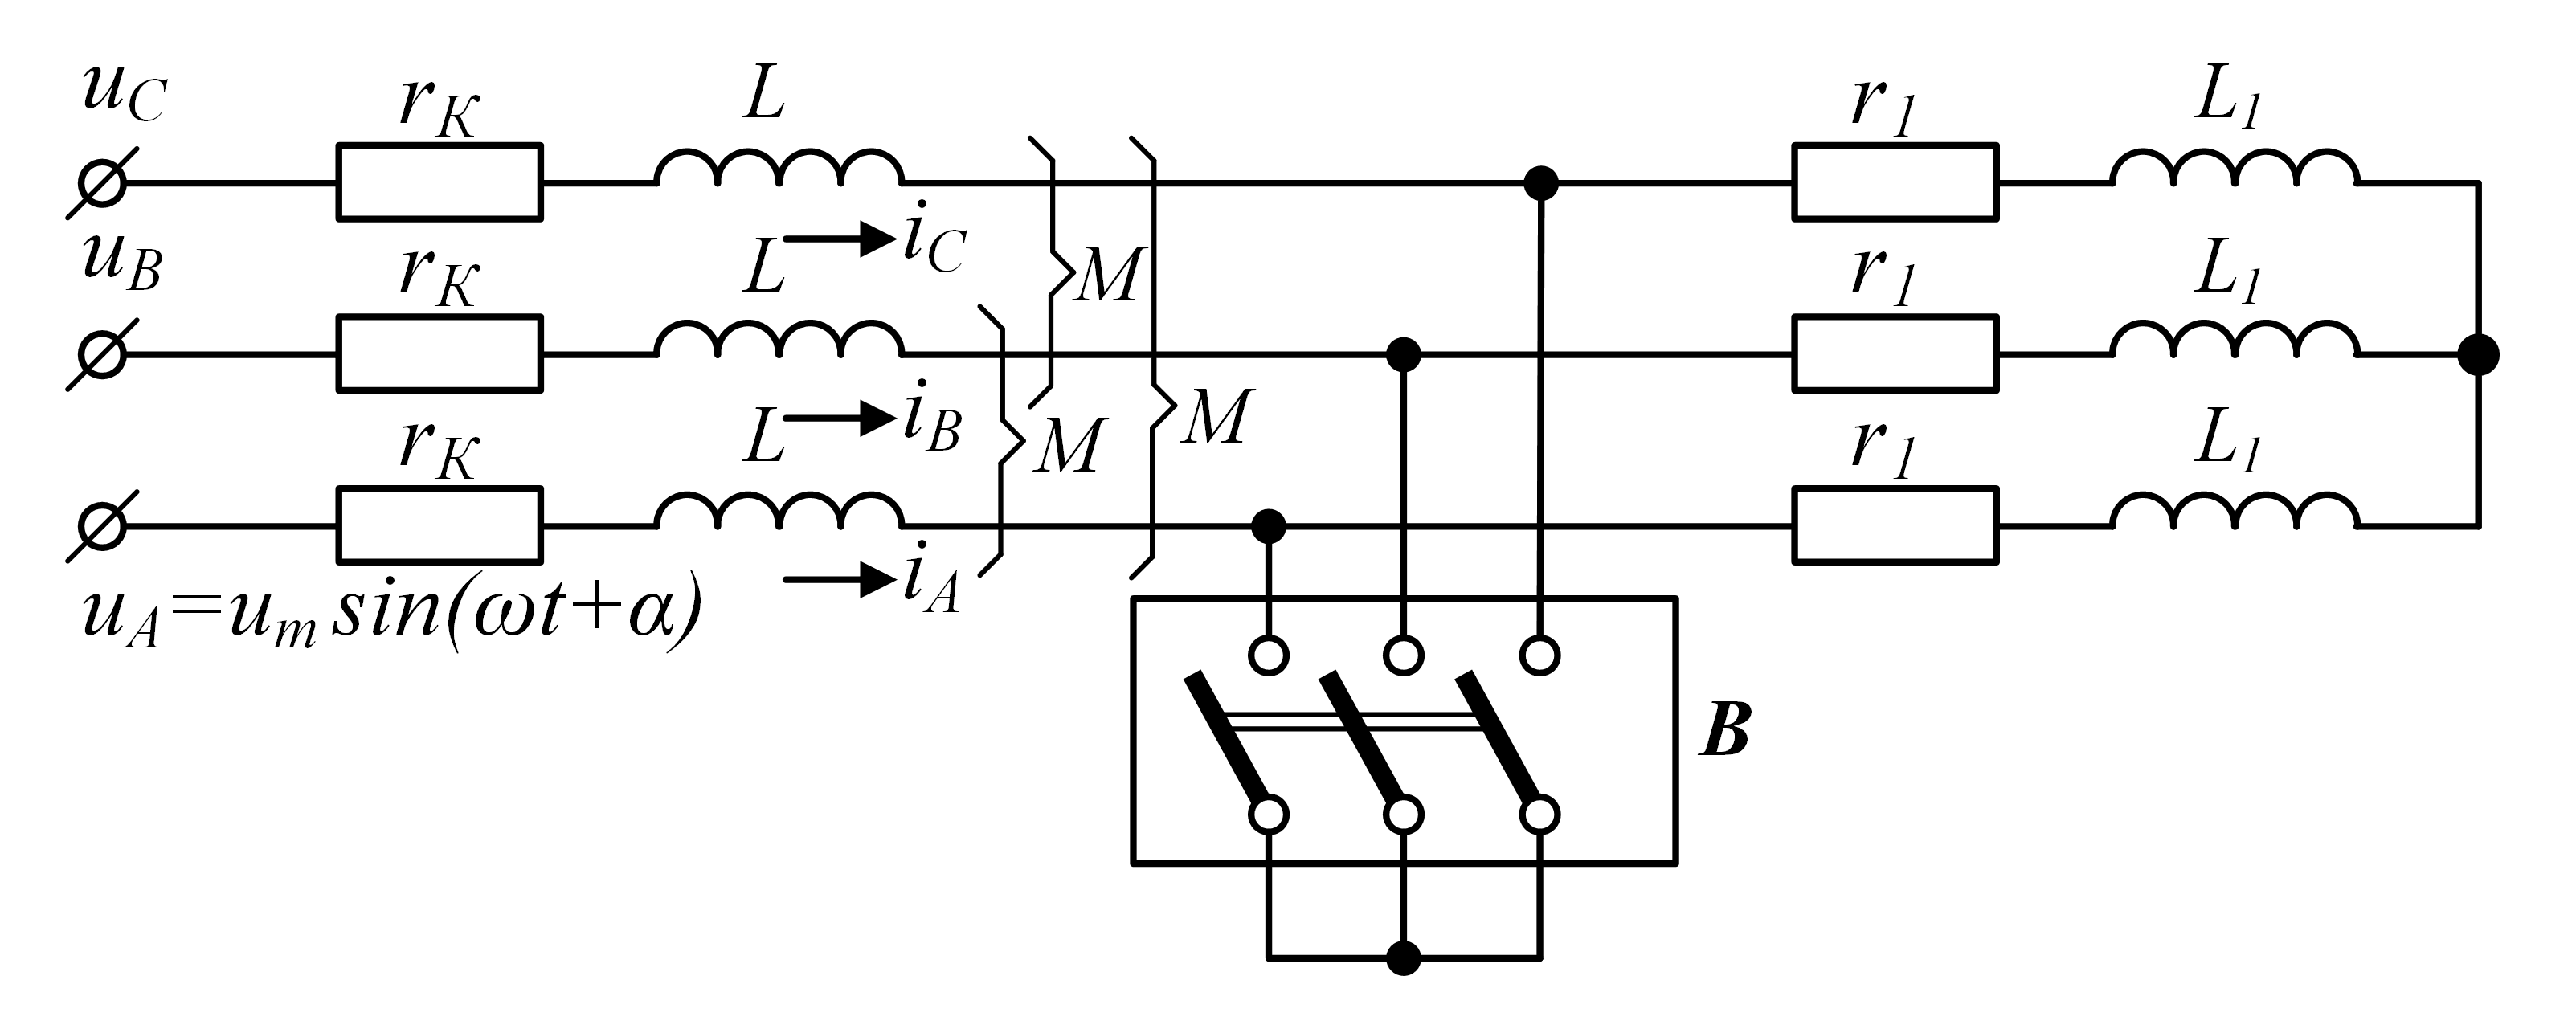
\includegraphics[width=0.9\linewidth]{pic/3-1}}
	\caption{Простейшая трехфазная электрическая цепь.}
	\label{ris:3-1 simple_3_phase_circut}
\end{figure}

Пусть векторы $ \overset{\;.}{U}_A $, $ \overset{\;.}{U}_B $, $ \overset{\;.}{U}_C $, $ \overset{\;.}{I}_A $, $ \overset{\;.}{U}_B $, $ \overset{\;.}{U}_C $ (рис.~\ref{ris:3-2 diagram})
характеризуют предшествующий режим рассматриваемой цепи, а вертикаль \textit{tt} является неподвижной линией времени, т.~е. мгновенные значения отдельных величии определяются проекциями на эту линию соответствующих вращающихся векторов. Момент возникновения короткого замыкания будем фиксировать значением угла $ \alpha $ (т.~е. \so{фазой включения}) между вектором напряжения фазы \textit{A} и горизонталью. (рис.~\ref{ris:3-2 diagram}.

После включения выключателя \textit{В} цепь рис.~\ref{ris:3-1 simple_3_phase_circut} распадается на два независимых друг от друга участка. Участок с $ r_1 $ и $ L_1 $ оказывается зашунтированным коротким замыканием и ток в нем будет поддерживаться лишь до тех пор, пока запасенная в индуктивности $ L_1 $ энергия магнитного потока не перейдет в тепло, поглощаемое активным сопротивлением $ r_1 $.

Дифференциальное уравнение равновесия в каждой фазе этого участка имеет вид:

\begin{equation}
	0 = ir_1 + L_1 \frac{di}{dt}.
	\label{eq:3-1 diff_ur}
\end{equation}

Его решение общеизвестно:

\begin{equation}
	i = i_0 e^{-t / T_{\text{а}1}}; %TODO: Проверить формулу, какая-то черка в степени
	\label{eq:3-2 diff_solve}
\end{equation}

оно показывает, что здесь имеется лишь свободный ток, который затухает по экспоненте с постоянной времени

\begin{equation}
	T_{\text{а}1} = \frac{L_1}{r_1} = \frac{x_1}{\omega r_1}, \textit{~сек}.
	\label{eq:3-3 T_a1}
\end{equation}

Начальное значение свободного тока в каждой фазе зашунтированного участка цепи, очевидно, равно предшествовавшему мгновенному значению тока, поскольку в цепи с индуктивностью не может произойти внезапного (скачком) изменения тока. В общем случае свободные токи в фазах различны, хотя их затухание, разумеется, происходит с одной и той же постоянной времени. В одной из фаз свободный ток может вообще отсутствовать, если в момент возникновения короткого замыкания предшествовавший ток в этой фазе проходил через нуль; при этом свободные токи в двух других фазах будут одинаковы по величине, но противоположны по направлению.

На рис.~\ref{ris:3-3} слева приведены кривые изменения фазных токов в зашунтированном участке рассматриваемой цени, с учетам, что короткое замыкание произошло в момент, отвечающий положению векторов на рис.~\ref{ris:3-2 diagram}.

\begin{floatingfigure}[lflt]{0.45\linewidth}
	\centering
	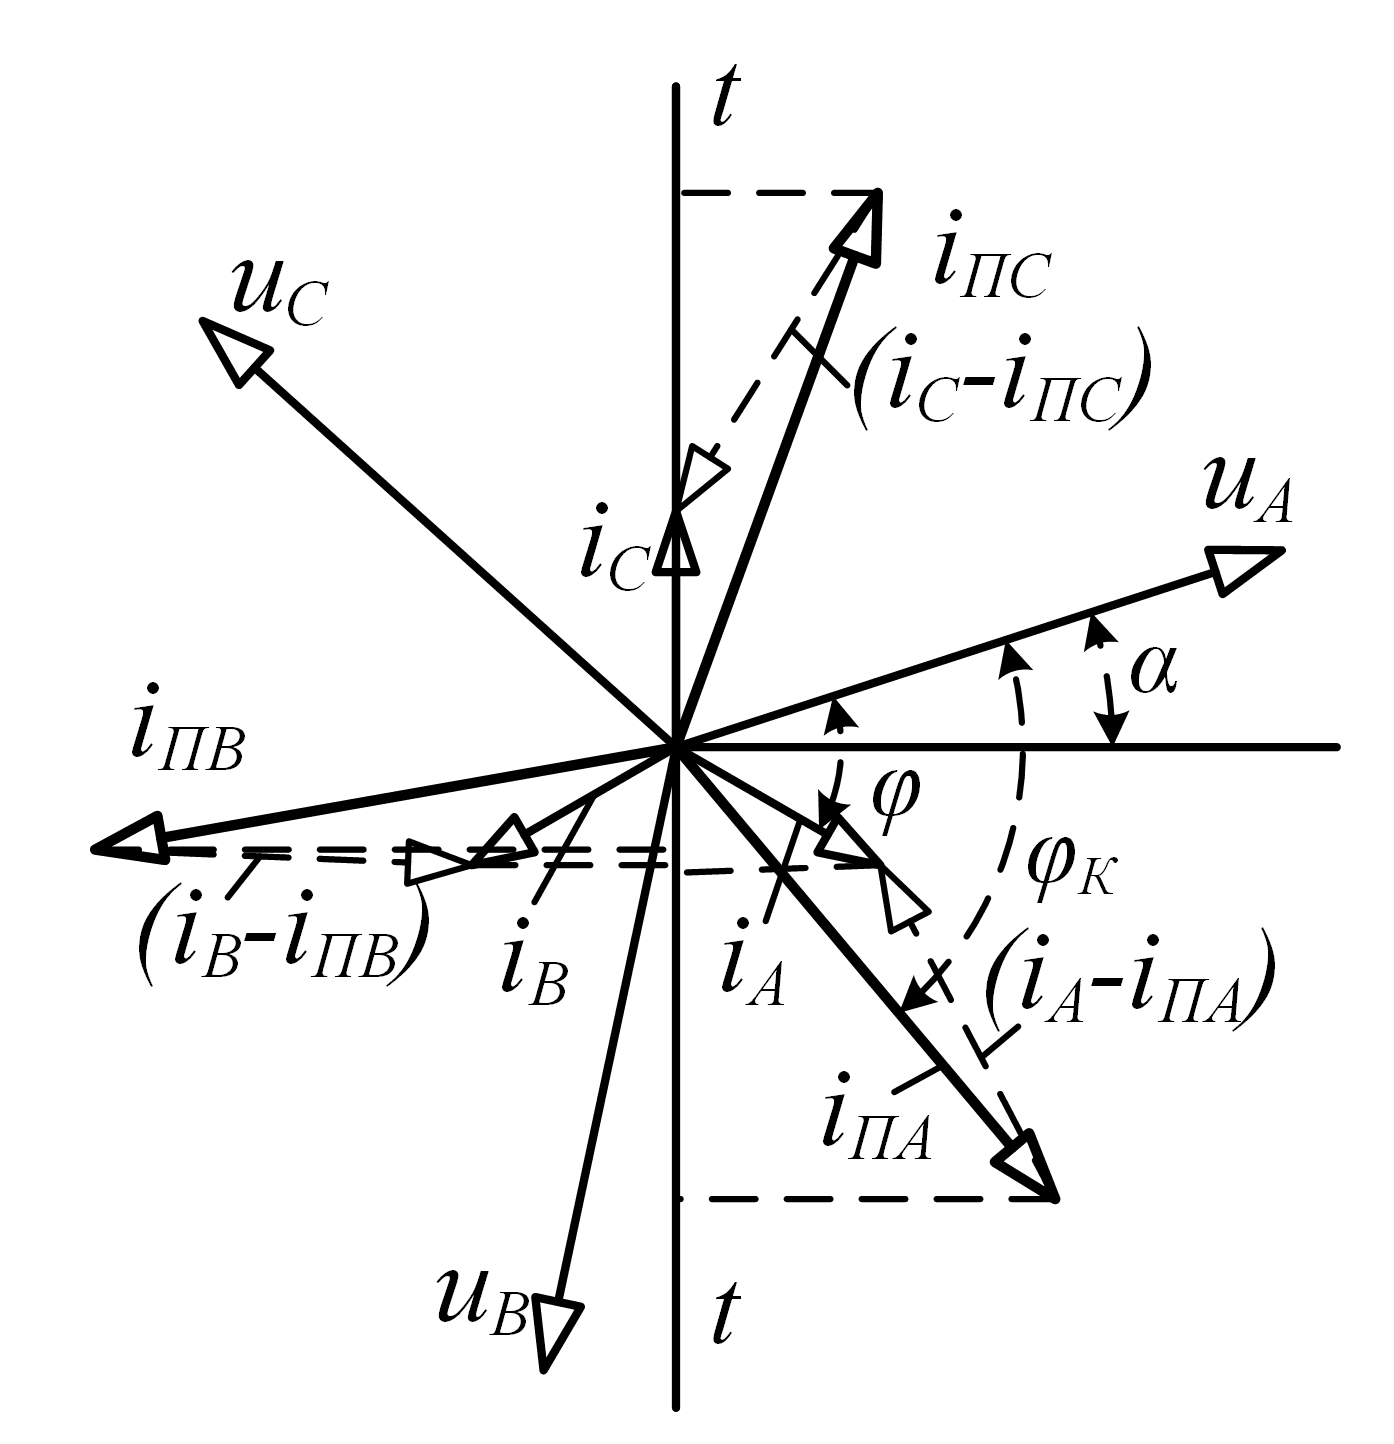
\includegraphics[width=0.40\linewidth]{pic/3-2}
	\caption{Векторная диаграмма для начального момента трехфазного короткого замыкания.}
	\label{ris:3-2 diagram}
\end{floatingfigure}

\begin{small}
	Напомним, что подкасательная в любой точке экспоненты\footnote{Обычно используют начальную часть экспоненты, где скорость изменения соответствующей величины больше и поэтому можно точнее провести касательную.} в принятом для оси времени масштабе дает значение постоянной времени, с которой происходит изменение экспоненты (рис.~\ref{ris:3-3}). Имея в виду, что при $ t = T_{\text{а}} $ значение $ e^{-1} = 0,368 $, постоянную $ T_{\text{а}} $ обычно трактуют как время, в течение которого переменная величина снижается до 0,368 своего начального значения; при этом за начальную может быть принята любая точка кривой.
	
\end{small}

%TODO: Рисунок оказывается перед 3-2 ??!!
\begin{figure}
	\center{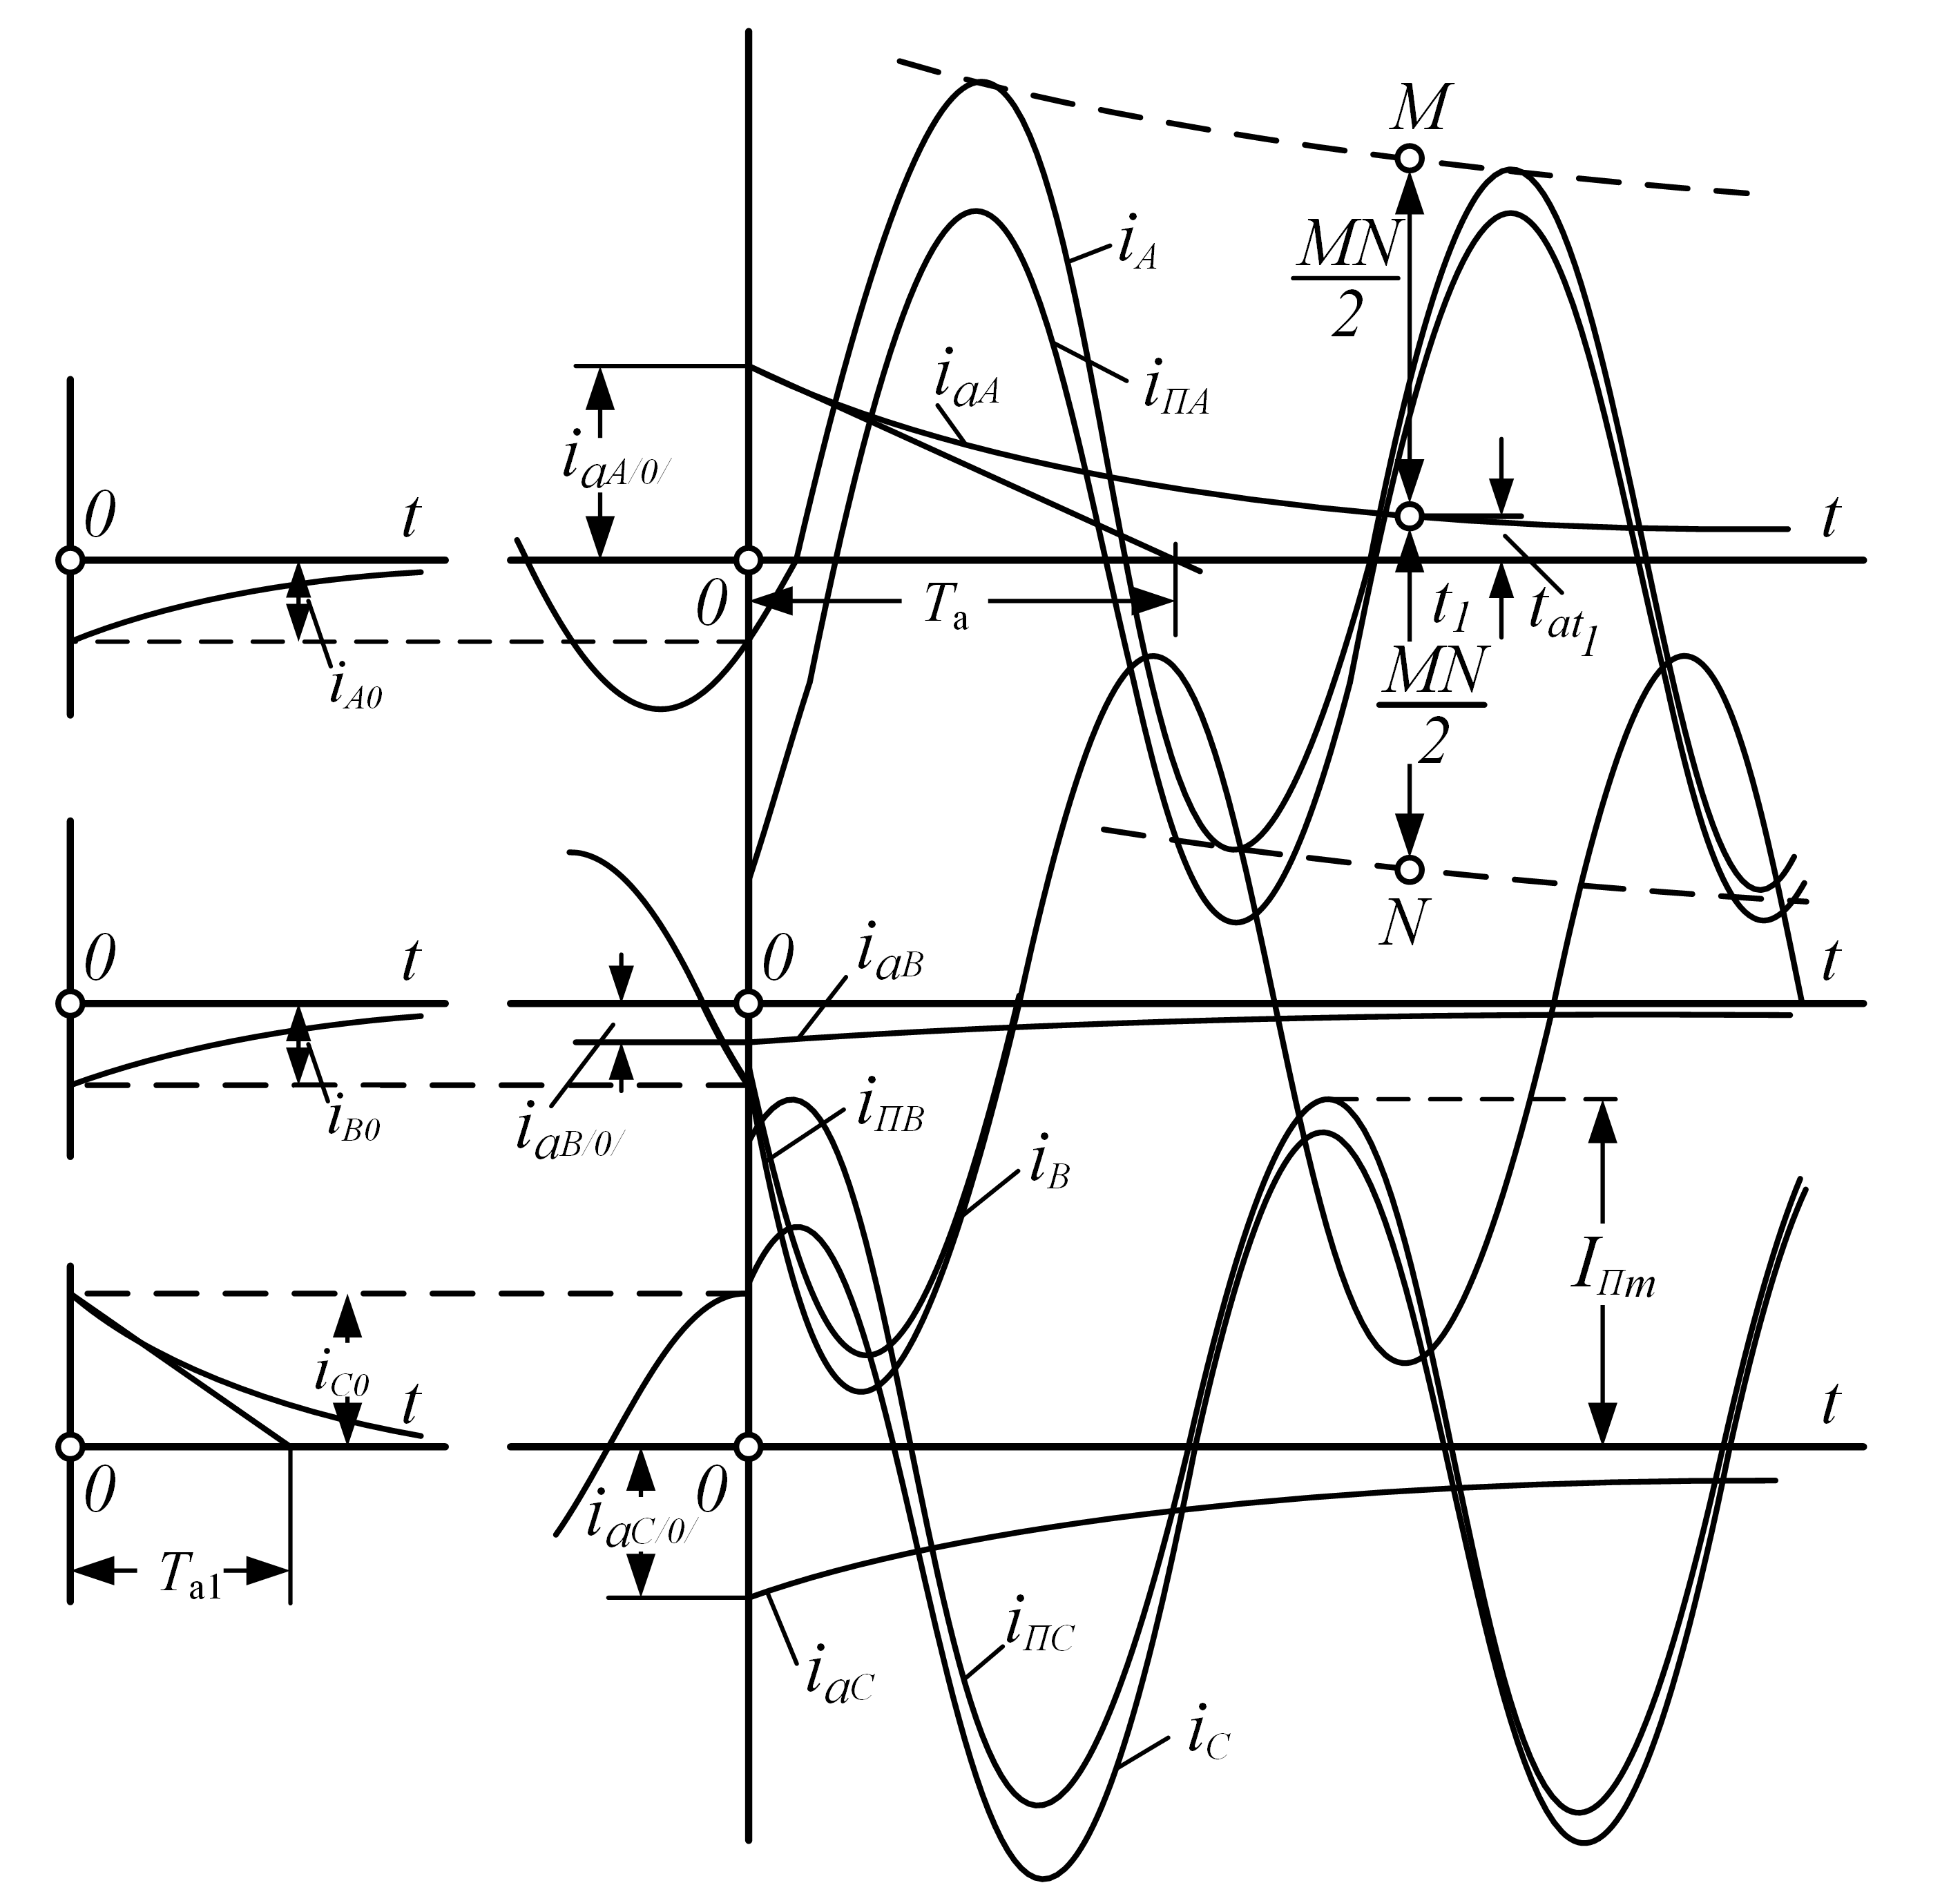
\includegraphics[width=0.85\linewidth]{pic/3-3}}
	\caption{Осциллограммы токов в фазах при внезапном трехфазном коротком замыкании в простейшей электрической цепи.}
	\label{ris:3-3}
\end{figure}

Перейдем теперь к участку цепи, который остался присоединенным к источнику. Здесь помимо свободного тока будет новый принужденный ток, величина которого, очевидно, больше предыдущего и сдвиг по фазе которого в общем случае иной. Допустим, что векторы $ I_{\text{П}A} $, $ I_{\text{П}B} $, $ I_{\text{П}C} $ (рис.~\ref{ris:3-2 diagram}) отвечают новому установившемуся режиму данного участка цепи.

Дифференциальное уравнение равновесия для любом фазы, например фазы \textit{А}, этого участка

\begin{equation*}
	u_A = i_A r_{\text{К}} + L \frac{di_A}{dt} + M \frac{di_B}{dt} + M \frac{di_C}{dt},
\end{equation*}

имея ввиду, что $ (i_B + i_C) = -i_A $, можно представить (опуская индекс фазы) как

\begin{equation}
    \label{eq:3-1a u}
	u = i r_{\text{К}} + L_{\text{К}} \frac{di}{dt},
	\tag{\ref*{eq:3-1 diff_ur}а}
\end{equation}

где $ L_{\text{К}} = (L - M) $ --- результирующая индуктивность фазы, т.~е. индуктивность с учетом влияния двух других фаз.

Решение (\ref{eq:3-1a u}) имеет вид:

\begin{equation}	
    \label{eq:3-2a i}
	i = \frac{U_m}{z_{\text{К}}} sin(\omega t + \alpha - \varphi_{\text{К}}) + i_{\text{а} | 0 |} e^{-t / T_{\text{а}}}
	\tag{\ref*{eq:3-2 diff_solve}а}	
\end{equation}

где $ z_{\text{К}} $ --- полное сопротивление присоединенного к источнику участка цепи или. короче, цепи короткого замыкания;

$ \varphi_{\text{К}} $ --- угол сдвига тока в этой цепи;
	
$ T_{\text{a}} $ --- постоянная времени цепи короткого замыкания, определяемая по (\ref{eq:3-3 T_a1}), где вместо $ L_1 $, $ x_1 $, $ r_1 $ следует ввести $ L_{\text{К}} $, $ x_{\text{К}} $, $ r_{\text{К}} $.

Первый член правой части (\ref{eq:3-2a i}) представляет периодическую слагающую тока, которая при рассматриваемых условиях является принужденным током с постоянной амплитудой $ I_{\text{П}m} = U_m / z_{\text{К}} $. Соответственно второй член представляет, как и раньше, затухающий по экспоненте свободный ток; его называют также апериодической слагающей тока. Начальное значение этой слагающей определяется из начальных условий, т.~е.

%TODO В этом месте в книге опечатка, формула названа 3-3, нумерация дальше отличается
\begin{equation}
	i_0 = i_{\text{п}~/0/} + i_{\text{а}~/0/},
	\label{eq:3-4 i_0}
\end{equation}

откуда после подстановки соответствующих выражений имеем:

\begin{equation}
	i_{\text{а}|0|} = I_m sin(\alpha - \varphi) - I_{\text{П}m} sin(\alpha - \varphi_{\text{К}}).
	\label{eq:3-5 i_a0}
\end{equation}

Поскольку токи $ i_{\text{П}} $, $ i_0 $ являются проекциями векторов $ \overset{\;.}{I}_{\text{П}m} $ и $ \overset{\;.}{I}_m $ на линию времени, то ток $ 	i_{\text{а}|0|} $ также можно рассматривать как проекцию вектора $ (\overset{\;.}{I}_m - \overset{\;.}{I}_{\text{П}m} $ на ту же линию (рис.~\ref{ris:3-2 diagram}). В зависимости от фазы включения $ \alpha $ начальное значение тока $ 	i_{\text{а}|0|} $ может изменяться от возможной наибольшей величины, когда вектор $ (\overset{\;.}{I}_m - \overset{\;.}{I}_{\text{П}m} $ параллелен линии времени, до нуля, когда этот вектор нормален к ней. В трехфазной системе такие частные условия, разумеется, могут быть лишь в одной из фаз.

\begin{figure}
	\center{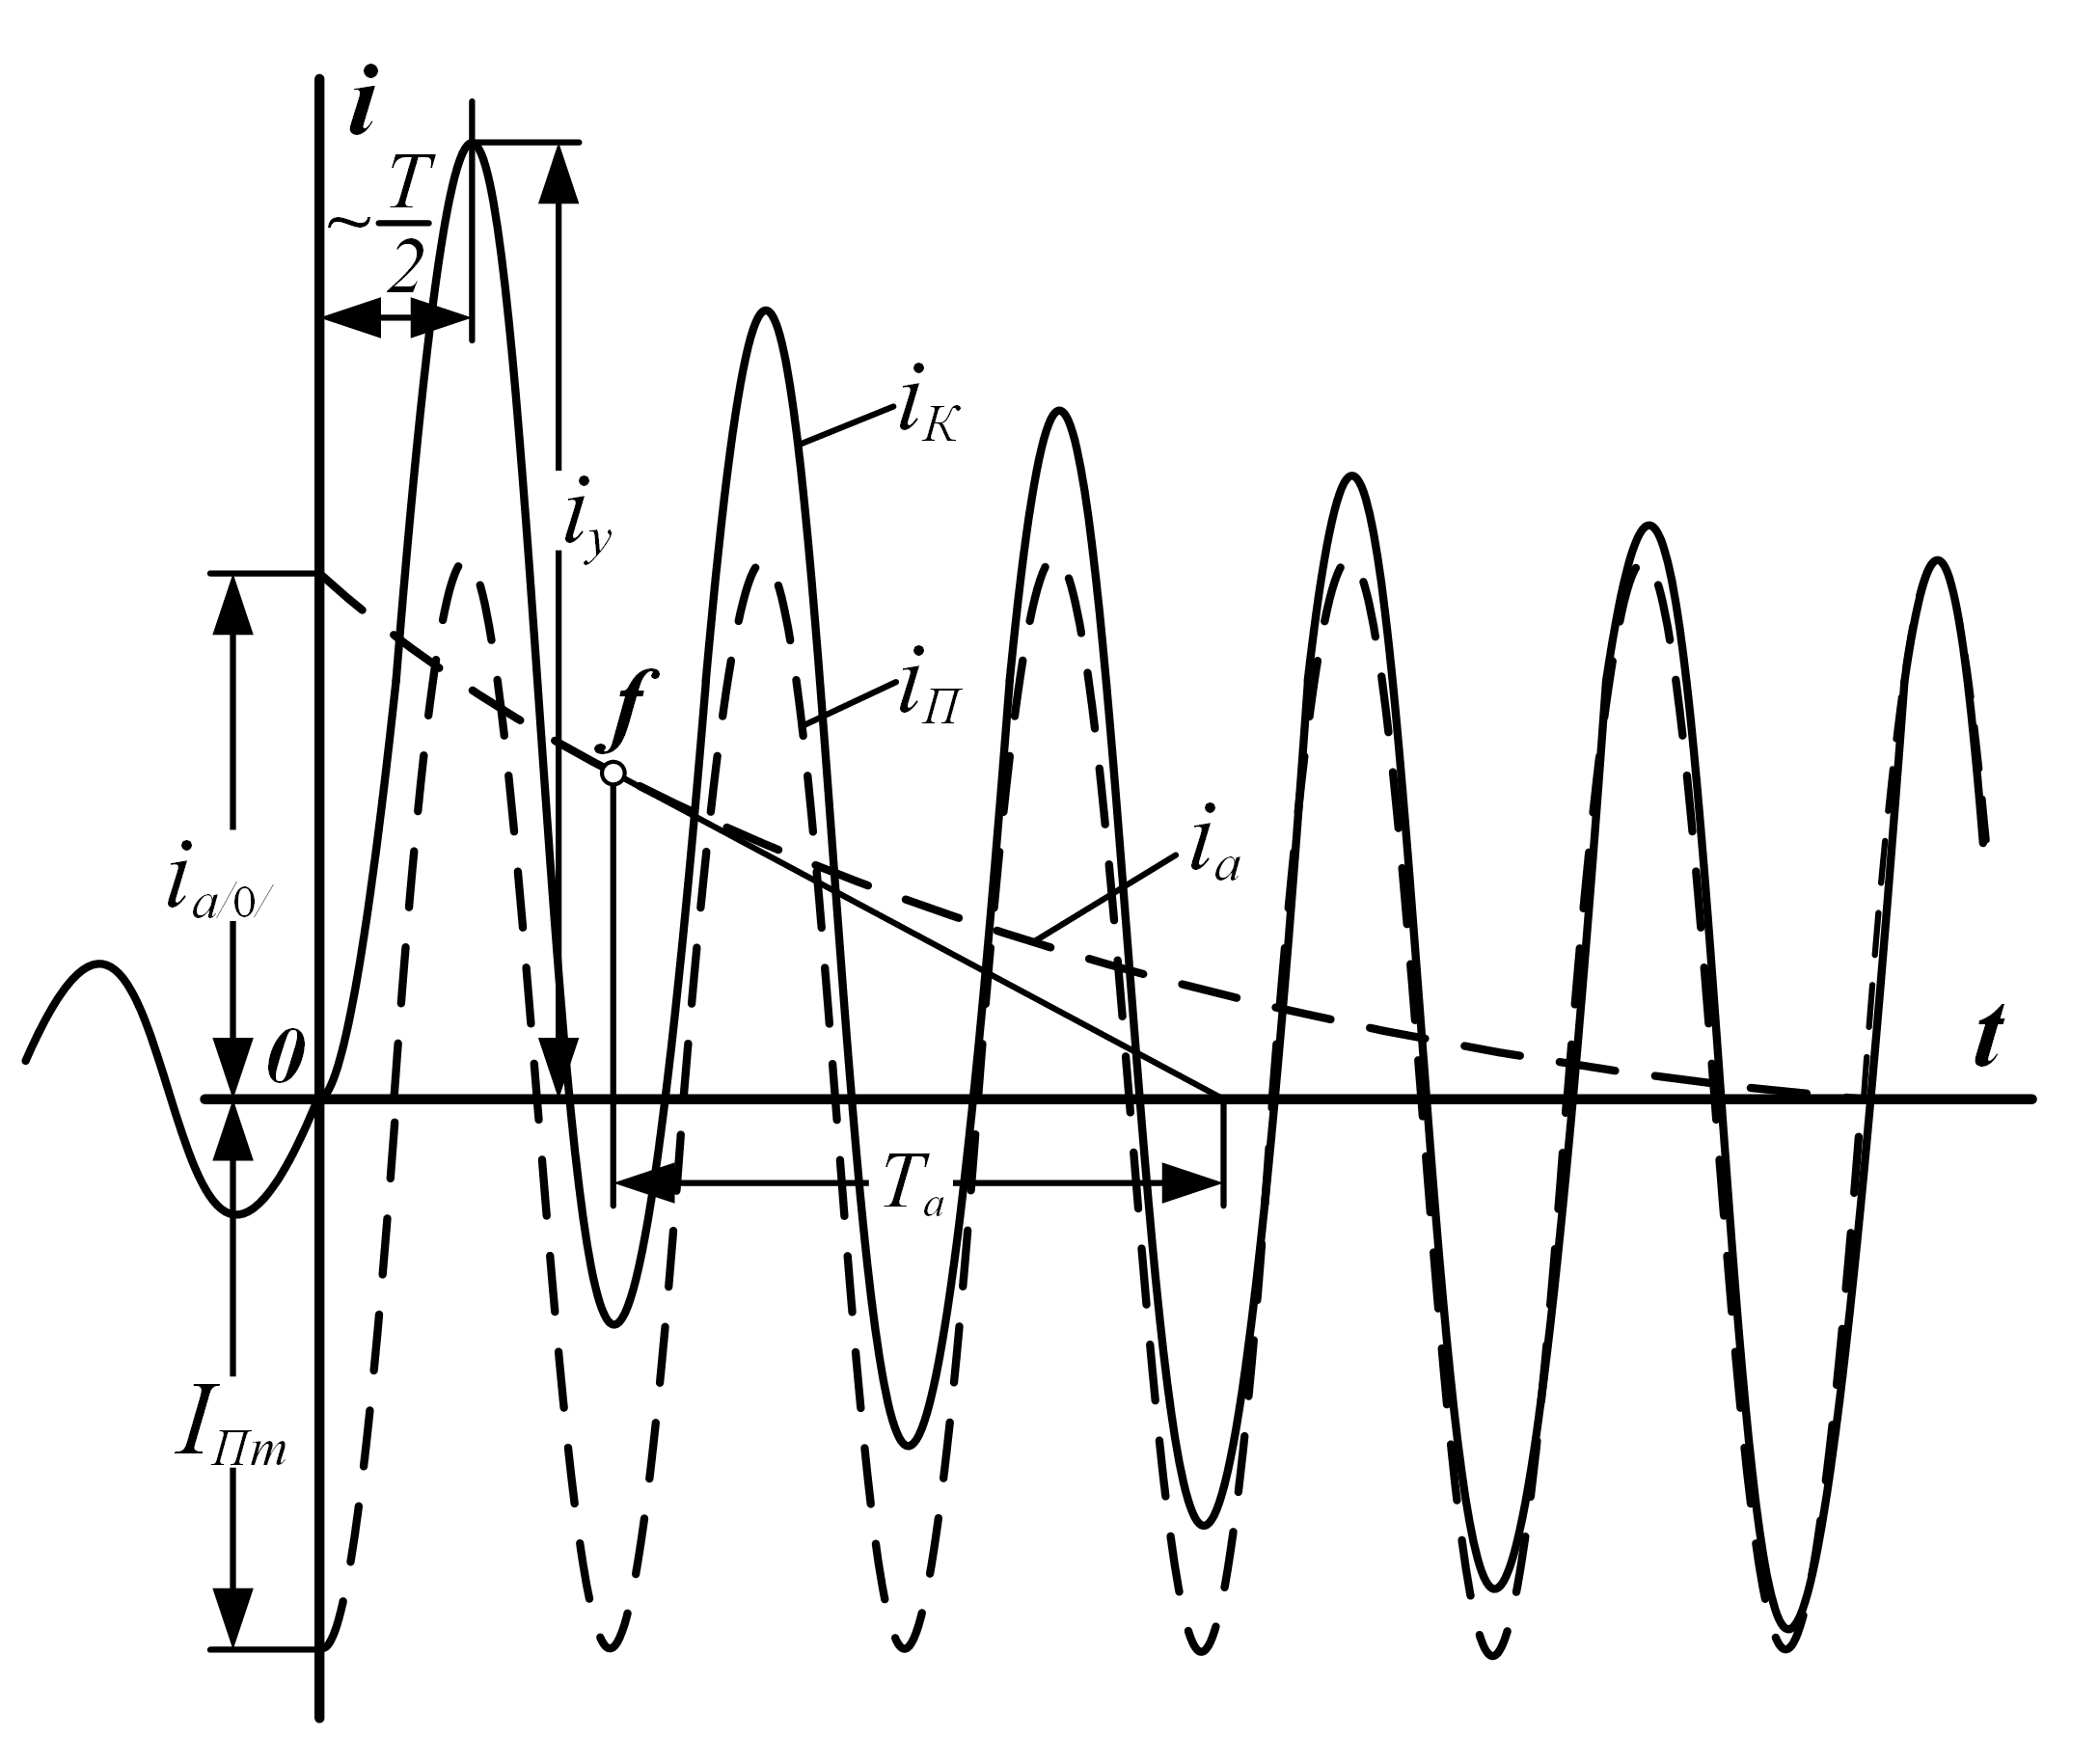
\includegraphics[width=0.85\linewidth]{pic/3-4}}
	\caption{Осциллограмма тока короткого замыкания при наибольшей апериодической слагающей.}
	\label{ris:3-4}
\end{figure}

На рис.~\ref{ris:3-3} справа представлены кривые изменения токов в фазах рассматриваемого участка при трехфазном коротком замыкании. Как видно, чем больше апериодическая слагающая тока, тем больше смещение кривой полного тока относительно оси времени. Эту слагающую можно рассматривать как криволинейную ось симметрии кривой полного тока, из которой ее легко выделить. Для этого нужно сначала провести огибающие по максимальным положительным и отрицательным значениям заданной кривой тока (см. пунктирные линии у кривой тока фазы \textit{А} на рис.~\ref{ris:3-3}). Каждая точка кривой апериодической слагающей лежит посредине вертикального отрезка между этими огибающими.

Из (\ref{ris:3-4}) и рис.~\ref{ris:3-2 diagram} следует, что наибольшее значение апериодической слагающей тока определяется не только фазой включения, но также предшествующим режимом цепи. Так, например, при отсутствии предшествующего тока в данной цепи величина 
при отсутствии величина $ i_{\text{а}/0/} $ может достигать амплитуды периодической слагающей, если в момент короткого замыкания эта слагающая проходит через свой положительный или отрицательный максимум (рис.~\ref{ris:3-4}). Обычно этот случай рассматривается как расчетный\footnote{Хотя возможны частные случаи, когда начальное значение апериодической слагающей тока превышает амплитуду периодической слагающей.}.

Важно отметить, что фаза включения, при которой возникает наибольшее значение апериодической слагающей, еще не предопределяет того, что именно при ней будет максимум мгновенного значения полного тока. В самом деле, из (\ref{eq:3-2a i}) и (\ref{eq:3-5 i_a0}) при отсутствии предшествующего тока ($ I_m = 0 $) следует, что полный ток в цепи короткого замыкания является функцией двух независимых переменных: времени $ t $ и фазы включения $ \alpha $ и выражается уравнением

\begin{equation}
	i = I_{\text{п}m} [sin( \omega t + \alpha - \varphi_{\text{к}}) - sin(\alpha - \varphi_{\text{к}}) e^{-t/T_{\text{a}}} ].
	\label{eq:3-6 i}
\end{equation}

%TODO: не пропущена ли здесь буква "к"
Приравняв к нулю частные производные этого уравнения, т.~е.

\begin{equation*}
	\frac{di}{dt} = \omega cos( \omega t + \alpha - \varphi_{\text{к}} ) + \frac{1}{T_{\text{a}}} sin( \alpha - \varphi_{\text{к}} ) e^{-t/T_{\text{a}}} = 0;
\end{equation*}

\begin{equation*}
	\frac{di}{d \alpha} = cos( \omega t + \alpha - \varphi_{\text{к}} ) - cos( \alpha - \varphi_{\text{к}} ) e^{-t/T_{\text{a}}} = 0,
\end{equation*}

и совместно решив эти уравнения, найдем, что максимум тока наступает при

\begin{equation*}
	tg( \alpha - \varphi_{\text{к}} ) = -\omega T_{\text{a}} = - \frac{x_{\text{к}}}{r_{\text{к}}} = tg( -\varphi_{\text{к}}).
\end{equation*}

т.~е. при $ \alpha = 0 $.

Следовательно, в предварительно разомкнутой цепи с $ r $ и $ L $ максимум мгновенного значения полного тока при коротком замыкании наступает, если в момент возникновения короткого
%TODO: пропущено слово "замыкания"
замыкания напряжение источника проходит через нуль.

Для цепей с преобладающей индуктивностью $ \varphi_{\text{к}} \approx 90^\circ $. поэтому условие возникновения наибольшей апериодической слагающей и условие, при котором достигается максимум мгновенного значения полного тока очень близки друг к другу. Поэтому в практических расчетах максимальное мгновенное значение полного тока короткого замыкания, которое называют \so{ударным током короткого замыкания $ i_{\text{у}} $},   обычно находят при наибольшем значении апериодической слагающей (рис.~\ref{ris:3-4}), считая, что он наступает приблизительно через полпериода, что при $ f = 50 \textit{~гц} $ составляет около 0,01~\textit{сек} с возникновения короткого замыкания.

Таким образом, выражение для ударного тока короткого замыкания можно записать в следующем виде:

\begin{equation}
	i_{\text{у}} = I_{\text{п}m} + I_{\text{п}m} e^{-0,01 / T_{\text{а}}} = k_{\text{у}} I_{\text{п}m},
	\label{eq:3-7 i_y}
\end{equation}

где

\begin{equation}
	k_{\text{у}} = 1 + e^{-0,01 / T_{\text{а}}},
	\label{eq:3-8 k_y}
\end{equation}

который называют \so{ударным коэффициентом}, показывает превышение ударного тока над амплитудой периодической слагающей; его величина находится в пределах

\begin{equation*}
	1 < k_{\text{у}} < 2,
\end{equation*}

что соответствует предельным значениям $ T_{\text{а}} $, т.~е. $ T_{\text{а}} = 0 $ (при $ L_{\text{к}} = 0 $)  и $ T_{\text{а}} = \infty $ (при $ r_{\text{к}} = 0 $).

Естественно, чем меньше $ T_{\text{а}} $, тем быстрее затухает апериодическая слагающая и тем соответственно меньше ударный коэффициент. Влияние этой слагающей сказывается лишь в начальной стадии переходного процесса; в сетях и установках высокого напряжения она практически исчезает спустя 0,1--0,3~\textit{сек}, а в установках низкого напряжения она практически совсем незаметна.

Еще раз подчеркнем, что апериодические слагающие токов в фазах различны. Поэтому определение трехфазного короткого замыкания как симметричного, строго говоря, справедливо применительно к периодическим слагающим фазных токов.

\section{Действующие значения полных величин и их отдельных слагающих}

Прежде всего оговорим условность принятой терминологии. Она заключается в том, что \so{действующее значение}, например, \so{тока в произвольный момент переходного процесса}, будем  иметь в виду, что оно  определится  как среднеквадратичное значение за один период $ T $, в середине которого находится рассматриваемый момент. В соответствии с этим при известной зависимости $ i = f(t) $ для  действующего значения тока в момент $ t $ можно написать:

\begin{equation}
	I_t = \sqrt{ \frac{1}{T} \int_{t-T/2}^{t+T/2} i^2 dt }.
	\label{eq:3-9 I_t}
\end{equation}

Зависимость $ i = f(t) $ в общем случае очень сложна. Поэтому для упрощения подсчета $ I_t $ принимают, что за рассматриваемый период обе слагающие тока не изменяются, т.~е. амплитуда периодической слагающей и апериодическая слагающая неизменны, каждая из них равна своему значению в данный момент $ t $. Такое допущение относительно периодической слагающей делают, когда источником является генератор конечной мощности; для условий же §\ref{sec:3-2 trekhfaznoe_korotkoe_zamykanie_v_nerazvetvlennoi_tcepi} постоянство амплитуды соблюдается.

\begin{figure}
	\center{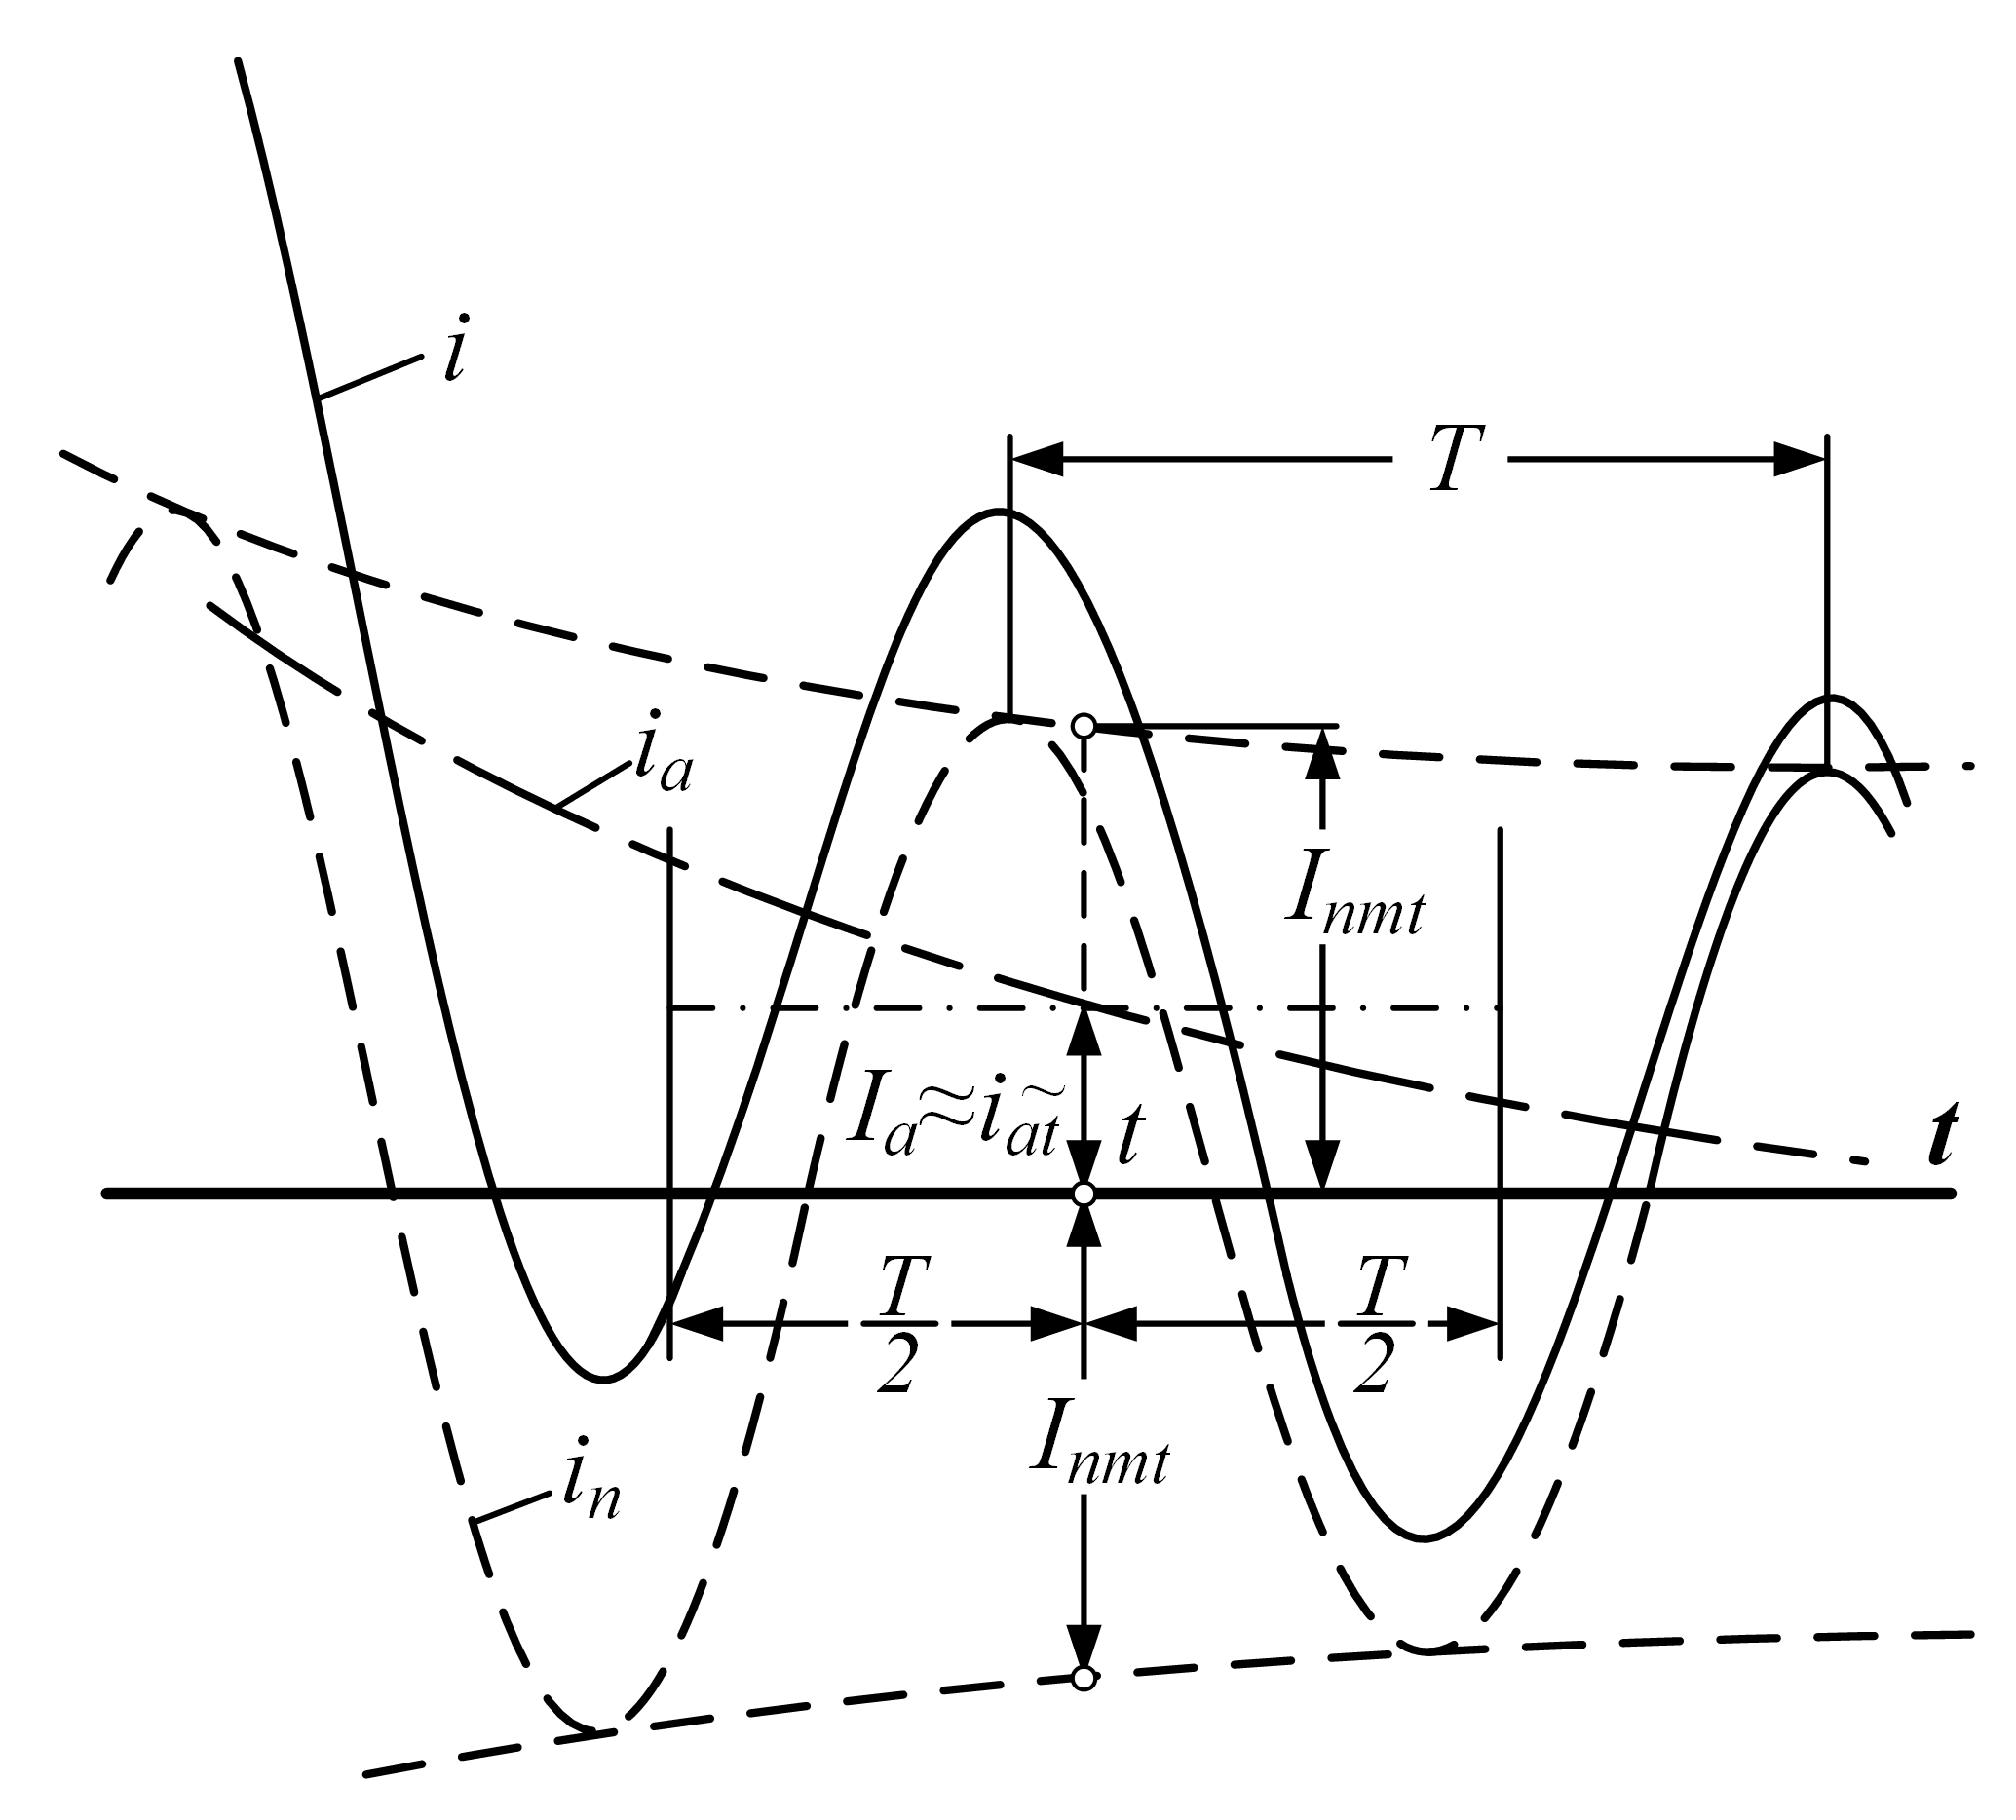
\includegraphics[width=0.85\linewidth]{pic/3-5}}
	\caption{К определению действующего значения тока в переходном процессе.}
	\label{ris:3-5}
\end{figure}

Сказанное иллюстрирует рис.~\ref{ris:3-5}, где для общности принято, что амплитуда периодической слагающей тока изменяется. Для заданного момента $ t $ амплитуду этой слагающей определяют по соответствующей огибающей (см.~пунктирные линии); при этом действующее значение рассматриваемой слагающей в этот момент находят как

\begin{equation}
	I_{\text{п}t} = I_{\text{п}mt} / \sqrt{2}.
	\label{eq:3-10 I_nt}
\end{equation}

Соответственно действующее значение апериодической слагающей за один период при принятом допущении равно ее мгновенному значению в момент, находящийся посредине данного периода (рис.~\ref{ris:3-5}) т.~е.

\begin{equation}
	I_{\text{a}t} = i_{\text{a}t}.
	\label{eq:3-11 I_at}
\end{equation}

Действующее значение полного тока в тот же момент будет:

%TODO: Проверить на счет точки над первой I под корнем
\begin{equation}
	I_t = \sqrt{I^2_{\text{п}t} + I^2_{\text{a}t}},
	\label{eq:3-12 I_t}
\end{equation}

т.~е. оно определяется знакомым выражением для действующего значения несинусоидального тока.

Точность определения по (\ref{eq:3-12 I_t}) вполне удовлетворяет требованиям практики.

\begin{floatingfigure}[rflt]{0.45\linewidth}
	\centering
	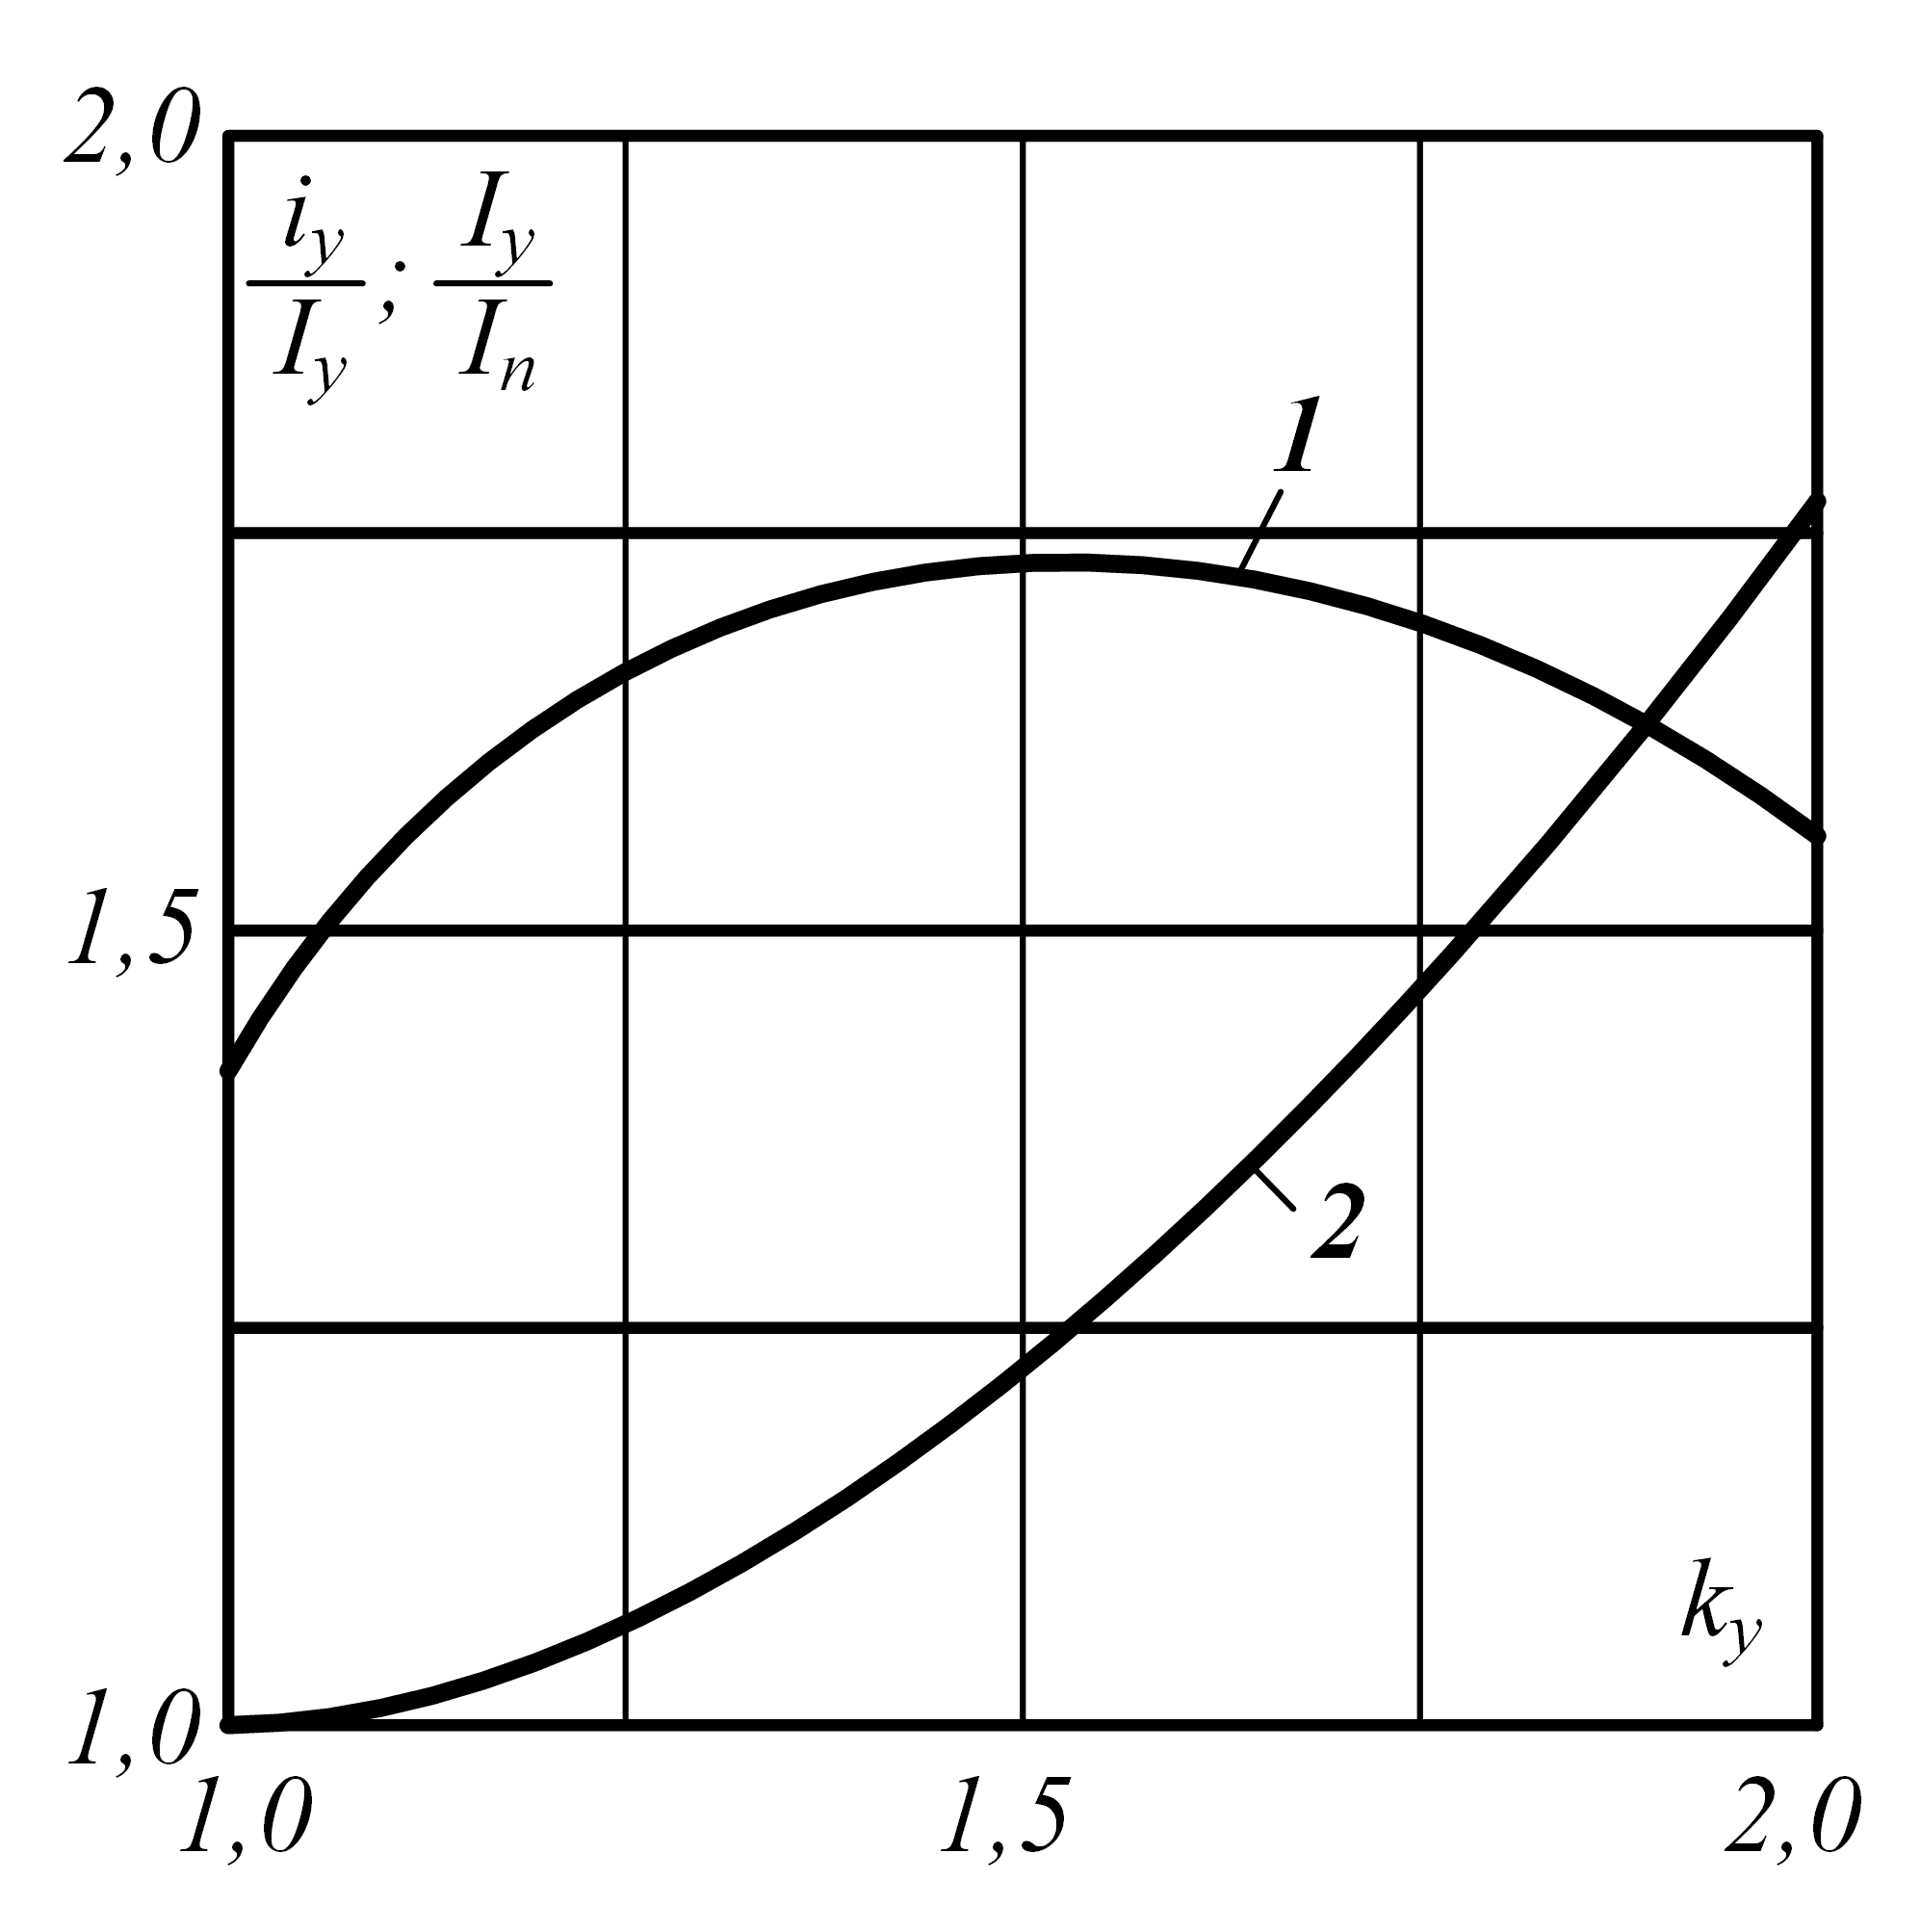
\includegraphics[width=0.43\linewidth]{pic/3-6}
	\caption{Кривые изменения отношений $ i_y / I_y $ (кривая \textit{1}) и $ I_y / I_{\text{п}} $ (кривая \textit{2}) в зависимости от ударного коэффициента $ k_y $.}
	\label{ris:3-6 I}
\end{floatingfigure}

\so{Наибольшее действующее значение полного тока короткого замыкания $ I_y $} имеет место за первый период  переходного процесса. При условии, когда $ i_{\text{a}}/0/ = I_{\text{п}m} $, его можно определить по (\ref{eq:3-12 I_t}), придав последнему следующий вид:

\begin{equation}
	I_y = \sqrt{I^2_{\text{п}} + [(k_y - 1) \sqrt{2} I_{\text{п}}]^2} = I_{\text{п}} \sqrt{1 + 2(k_y-1)^2},
	\label{eq:3-13 I_y}
\end{equation}

где $ k_y $ --- ударный коэффициент.

Согласно указанным выше пределам изменений $ k_y $ величина отношения $ I_y / I_{\text{п}} $ находится в пределах

\begin{equation*}
	1 < \frac{I_y}{I_{\text{п}}} < \sqrt{3}.
\end{equation*}

На рис.~\ref{ris:3-6 I} показаны кривые изменения отношений $ I-y / I_{\text{п}} $ и $ i_y / I_y $ в функции $ k_y $. Как видно, отношение $ i_y / I_y $ изменяется в сравнительно узких пределах и его максимум ($ \sqrt{3} $) наступает при $ k_y = 1,5 $.


\section{Приближенное решение}

Представим выражение для периодической слагающей тока короткого замыкания в несколько ином виде, т.~е.

\begin{equation*}
	I_{\text{п}m} = \frac{U_m}{z_{\text{к}}} = \frac{U_m}{x_{\text{к}} \sqrt{1 + c^2}} = \frac{I_{\text{п}m~(r_{\text{к}}=0)}}{\sqrt{1 + c^2}},
\end{equation*}                                                                      .

где $ I_{\text{п}m~(r_{\text{к}}=0)} = U_m / x_{\text{к}} $ --- значение той же слагающей при $ r_{\text{к}} = 0 $ и $ c = r_{\text{к}} / x_{\text{к}} $.

Таким образом, преувеличение периодической слагающей тока, вызванное пренебрежением $ r $, можно характеризовать отношением

\begin{equation}
	\frac{I_{\text{п}m~(r_{\text{к}}=0)}}{I_{\text{п}m}} = \sqrt{1 + c^2}.
	\label{eq:3-14 otn}
\end{equation}

Если считать, что это превышение не должно быть более 5\%, то из (\ref{eq:3-14 otn}) легко установить, что оно будет соблюдаться при

\begin{equation*}
	c \leq \sqrt{1,05^2 - 1} \approx 1/3,
\end{equation*}

т.~е. определение $ I_{\text{п}} $ можно производить без учета $ r_{\text{к}} $, когда $ r_{\text{к}} \leq x_{\text{к}} / 3 $. При этом, конечно, фаза данной слагающей тока получается искаженной: $ \varphi_{\text{к}} = 90^{\circ} $ вместо $ \varphi_{\text{к}} = 72^{\circ} $ при  $ r_{\text{к}} = x_{\text{к}} / 3 $. Что касается апериодической слагающей, то при $ r_{\text{к}} = 0 $ ее затухание вообще отсутствует и $ k_y = 2 $, в то время как при $ r_{\text{к}} = x_{\text{к}} / 3 $ имеем $ k_y = 1,37 $; преувеличение ударного тока уже составляет 53\%, а электродинамического эффекта --- в $ 1,53^2 \approx 2,5 $~раза. Аналогично нетрудно установить, что при тех же условиях преувеличение в наибольшем действующем значении полного тока короткого замыкания достигает 61\%.

\begin{floatingfigure}[rflt]{0.45\linewidth}
	\centering
	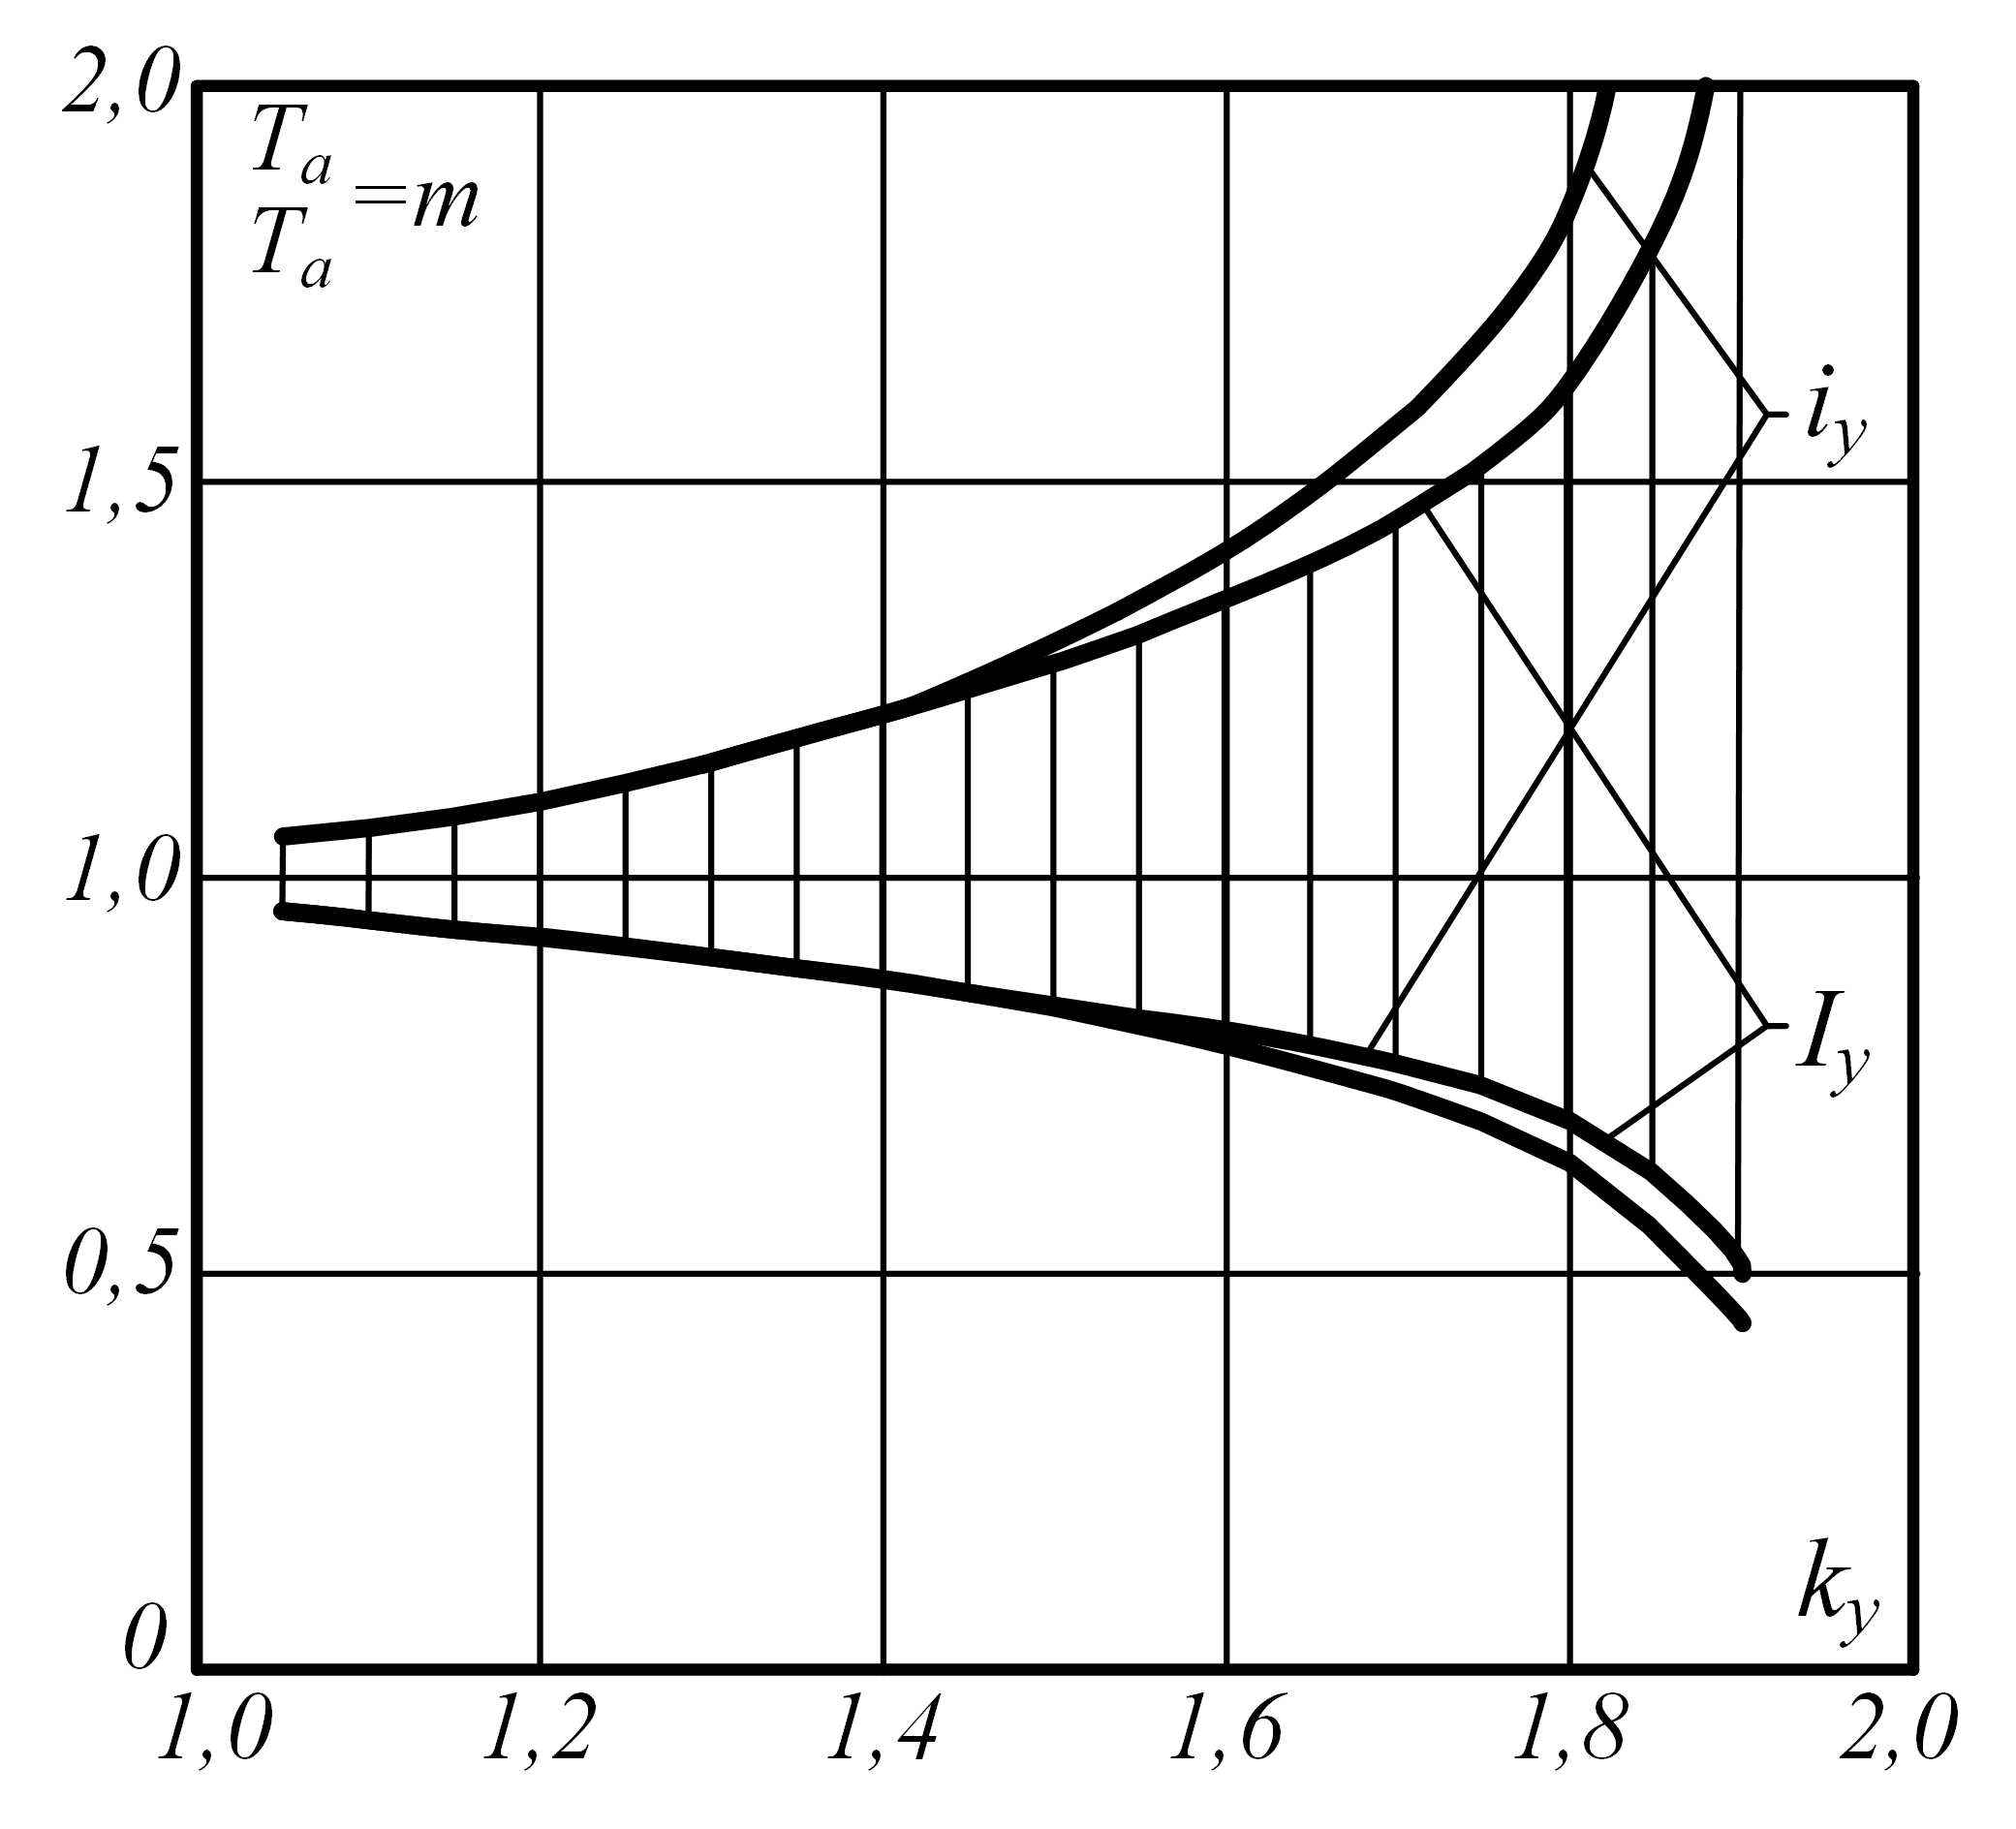
\includegraphics[width=0.40\linewidth]{pic/3-7}
	\caption{Кривые, ограничивающие зону времени $ T'_{\text{а}} $, при котором погрешность в токах $ i_y $ и $ I_y $ не превышает $ \pm5 \% $.}
	\label{ris:3-7 diagram}
\end{floatingfigure}

Этот элементарный подсчет наглядно иллюстрирует, насколько одно и то же допущение может привести к резко отличающимся погрешностям в определении отдельных величин. Очевидно, достаточно правильная оценка апериодической слагающей и полных величин тока, в которых ее участие существенно, может быть получена при непременном учете активного сопротивления цепи. Последний можно сделать приближенно и даже в неявной форме путем использования некоторой средней величины постоянной времени $ T_{\text{а}} $ и соответствующего ей значения ударного коэффициента. Такое различие в принимаемых допущениях при практической оценке отдельных слагающих тока является одним из примеров той условности и как бы несогласованности, о чем отмечалось в ~§\ref{sec:2-1 osnovnye dopushcheniia}.

Используя (\ref{eq:3-7 i_y}) и (\ref{eq:3-13 I_y}), можно установить допустимые отклонения приближенной величины постоянной времени $ T_{\text{а}} $, при которых ошибки в определении ударного тока и наибольшего действующего значения тока короткого замыкания не выходили бы за пределы $ \pm5 \% $. Результаты такого подсчета приведены на рис.~\colorbox{red}{3-7}, где допускаемые по данному условию пределы $ m = T'_{\text{а}} / T_{\text{а}} $ ограничены соответствующими кривыми в зависимости от $ k_y $. При $ k_y = 1,8 $ постоянная времени $ T_{\text{а}} = 0,045 $~\textit{сек}; если приближенно вычисленная $ T'_{\text{а}} $ согласно данным рис.~\colorbox{red}{3-7} находится а пределах $ T'_{\text{а}} = (0,65 \div 1,83)~~T_{\text{а}} = 0,029 \div 0,082 $~\textit{сек}, то ошибка в ударном токе не превысит $ \pm5 \% $.

\section{Определение эквивалентной постоянной времени}

Для цепи, состоящей из последовательно соединенных элементов, определение постоянной времени $ T_{\text{а}} $ не представляет труда. Ее значение легко находится по формуле, аналогичной (\ref{eq:3-3 T_a1}), где под $ x_1 $ и $ r_1 $ следует понимать соответственно индуктивное и активное сопротивления всей короткозамкнутой цепи.

Иное положение имеет место в сложной разветвленной схеме. Нахождение свободного тока в любой ветви такой схемы является задачей, с которой читатель знаком из курса теоретических основ электротехники. Как известно, ее решение наиболее эффективно достигается путем применения преобразования Лапласа, т.~е. с использованием операторного метода.

При отсутствии кратных корней характеристического уравнения $ z(p)= 0 $ для свободного тока произвольной ветви в соответствии с известной формулой разложения имеем:

\begin{equation}
	\sum_{k=1}^{k=n}\frac{F_1 (p_{\text{k}})}{p_{\text{k}} F'_2(p_{\text{k}})} e^{p_{\text{k}}t} = I_{\text{a}1}e^{p_1t} + I_{\text{a}2}e^{p_2t} + \ldots + I_{\text{a}n}e^{p_nt},
	\label{eq:3-15 diff}
\end{equation}

где каждое из слагаемых представляет частный свободный ток.

Когда в схеме нет емкости, все корни характеристического уравнения являются вещественными отрицательными величинами и для них можно написать:

%TODO: Проверить формулу
\begin{equation*}
	p_1 = - 1 / T_{\text{a}1}; \hspace{1pc} p_2 = - 1 / T_{\text{a}2}; \hspace{1pc} \ldots; \hspace{1pc} p_n = - 1 / T_{\text{a}n},
\end{equation*}

где $ T_{\text{a}1}, T_{\text{a}2}, \ldots, T_{\text{a}n} $ --- постоянные времени свободных токов.

Начальные значения частных свободных токов $ I_{\text{a}1}, I_{\text{a}2}, \ldots, I_{\text{a}n} $, равно как и их постоянные времени, являются функциями параметров всех элементов схемы.

Такой общий строгий путь решения уже для маломальски сложной схемы требует большой вычислительной работы. Достаточно напомнить, что каждая параллельная ветвь с $ r $ и $ L $ увеличивает на один порядок степень характеристического уравнения. Поэтому для практических расчетов довольствуются более простым, приближенным решением, одно из которых состоит в замене (\ref{eq:3-15 diff}) одной экспонентой:

\begin{equation}
	I_{\text{a}t} = I_{\text{a/0/}}e^{-t/T_{\text{a.Э}}},
	\label{eq:3-16 exp}
\end{equation}

где $ T_{\text{a.Э}} $ --- некоторая эквивалентная постоянная времени, определяемая как

\begin{equation}
	T_{\text{a.Э}} = \frac{x_{\sum}}{\omega r_{\sum}},
	\label{eq:3-17 T_a}
\end{equation}

причем здесь $ x_{\sum} $ --- суммарное индуктивное сопротивление схемы, найденное при отсутствии всех активных сопротивлений ($ r = 0 $), и $ r_{\sum} $ --- суммарное активное сопротивление схемы при отсутствии всех индуктивных сопротивлений ($ x_{\sum} = 0 $). Такой искусственный прием определения $ T_{\text{a.Э}} $ сильно упрощает решение\footnote{Отметим, что такой упрощенный подсчет апериодической слагающей (вернее, $ T_{\text{a.Э}} $), в частности, принят в последнем американ	ском стандарте на выключатели высокого напряжения.}. При нем приблизительно соблюдается эквивалентность количества электричества в действительных и заменяемых условиях.

Что касается начального значения $ I_{\text{a/0/}} $ в (\ref{eq:3-16 exp}), то его легко определить по начальным условиям для данной ветви, поскольку начальное значение периодической слагающей тока нетрудно подсчитать, а предшествующий ток, как правило, известен.

При более грубых расчетах обычно не прибегают к подсчету $ T_{\text{a.Э}} $, а принимают для нее некоторое среднее значение в соответствии с принятым для данных условий ударным коэффициентом. Так, при $ k_{\text{у}} = 1,8 $ значение $ T_{\text{а}} = 0,045 $~\textit{сек}, которое считают одним и тем же для всех ветвей схемы.

\setcounter{example}{1}

\begin{small} % пример 3-1
	
	\vspace{1pc}
	\textit{Пример \ref*{chap:3 perehodnyi_protcess_v_prosteishikh_trekhfaznykh_tcepiakh}-\arabic{example}}.
	Для схемы, показанной в верхней части \colorbox{red}{рис. 3-8}, найти затухание свободных токов и эквивалентную постоянную времени. Сопротивления элементов выражены в операторной форме и	заданы в относительных единицах при некоторых базисных условиях.
	
	Определим результирующее операторное сопротивление схемы:
	
	\begin{equation*}
		z(p) = \frac{(1+15p)(1+3p)}{(1+15p)+(1+3p)} + (1+2p) = \frac{81p^2+40p+3}{2+18p}.
	\end{equation*}
	
	Из $ z(p) = 0 $, т.~е. их уравнения $ 81p^2+40p+3 = 0 $ находим корни:
	
	\begin{equation*}
		p_{1,2} = \frac{-40 \pm \sqrt{40^2 - 4,81 \cdot 3}}{2 \cdot 81},
	\end{equation*}
	
	%TODO: поправить звездочку под T
	т.~е. $	p_1 = -0,091  $; соответственно $ \underset{*}{T}_{\text{a1}} = \frac{-1}{-0,091} = 11 $; $ p_2 = -0,405 $; соответственно $ \underset{*}{T}_{\text{a2}} = \frac{-1}{-0,405} = 2,47 $.
	
	В именованных единицах эти постоянные времени будут:
	
	\begin{equation*}
		\underset{*}{T}_{\text{a1}} = \frac{11}{314} = 0,035 \text{~сек}
		\hspace{1pc}
		\underset{*}{T}_{\text{a2}} = \frac{2,47}{314} = 0,008 \text{~сек.}
	\end{equation*}
	
	Относительная величина свободного тока в общей ветви схемы пропорциональна результирующей операторной проводимости
	
	\begin{equation*}
		I_{\text{а}}(p) = Y(p) = 1/z(p) = \frac{2+18p}{81p^2 + 40p + 3} = \frac{F_1(p)}{F_2(p)}.
	\end{equation*}
	
	\begin{figure}[h]
		\center{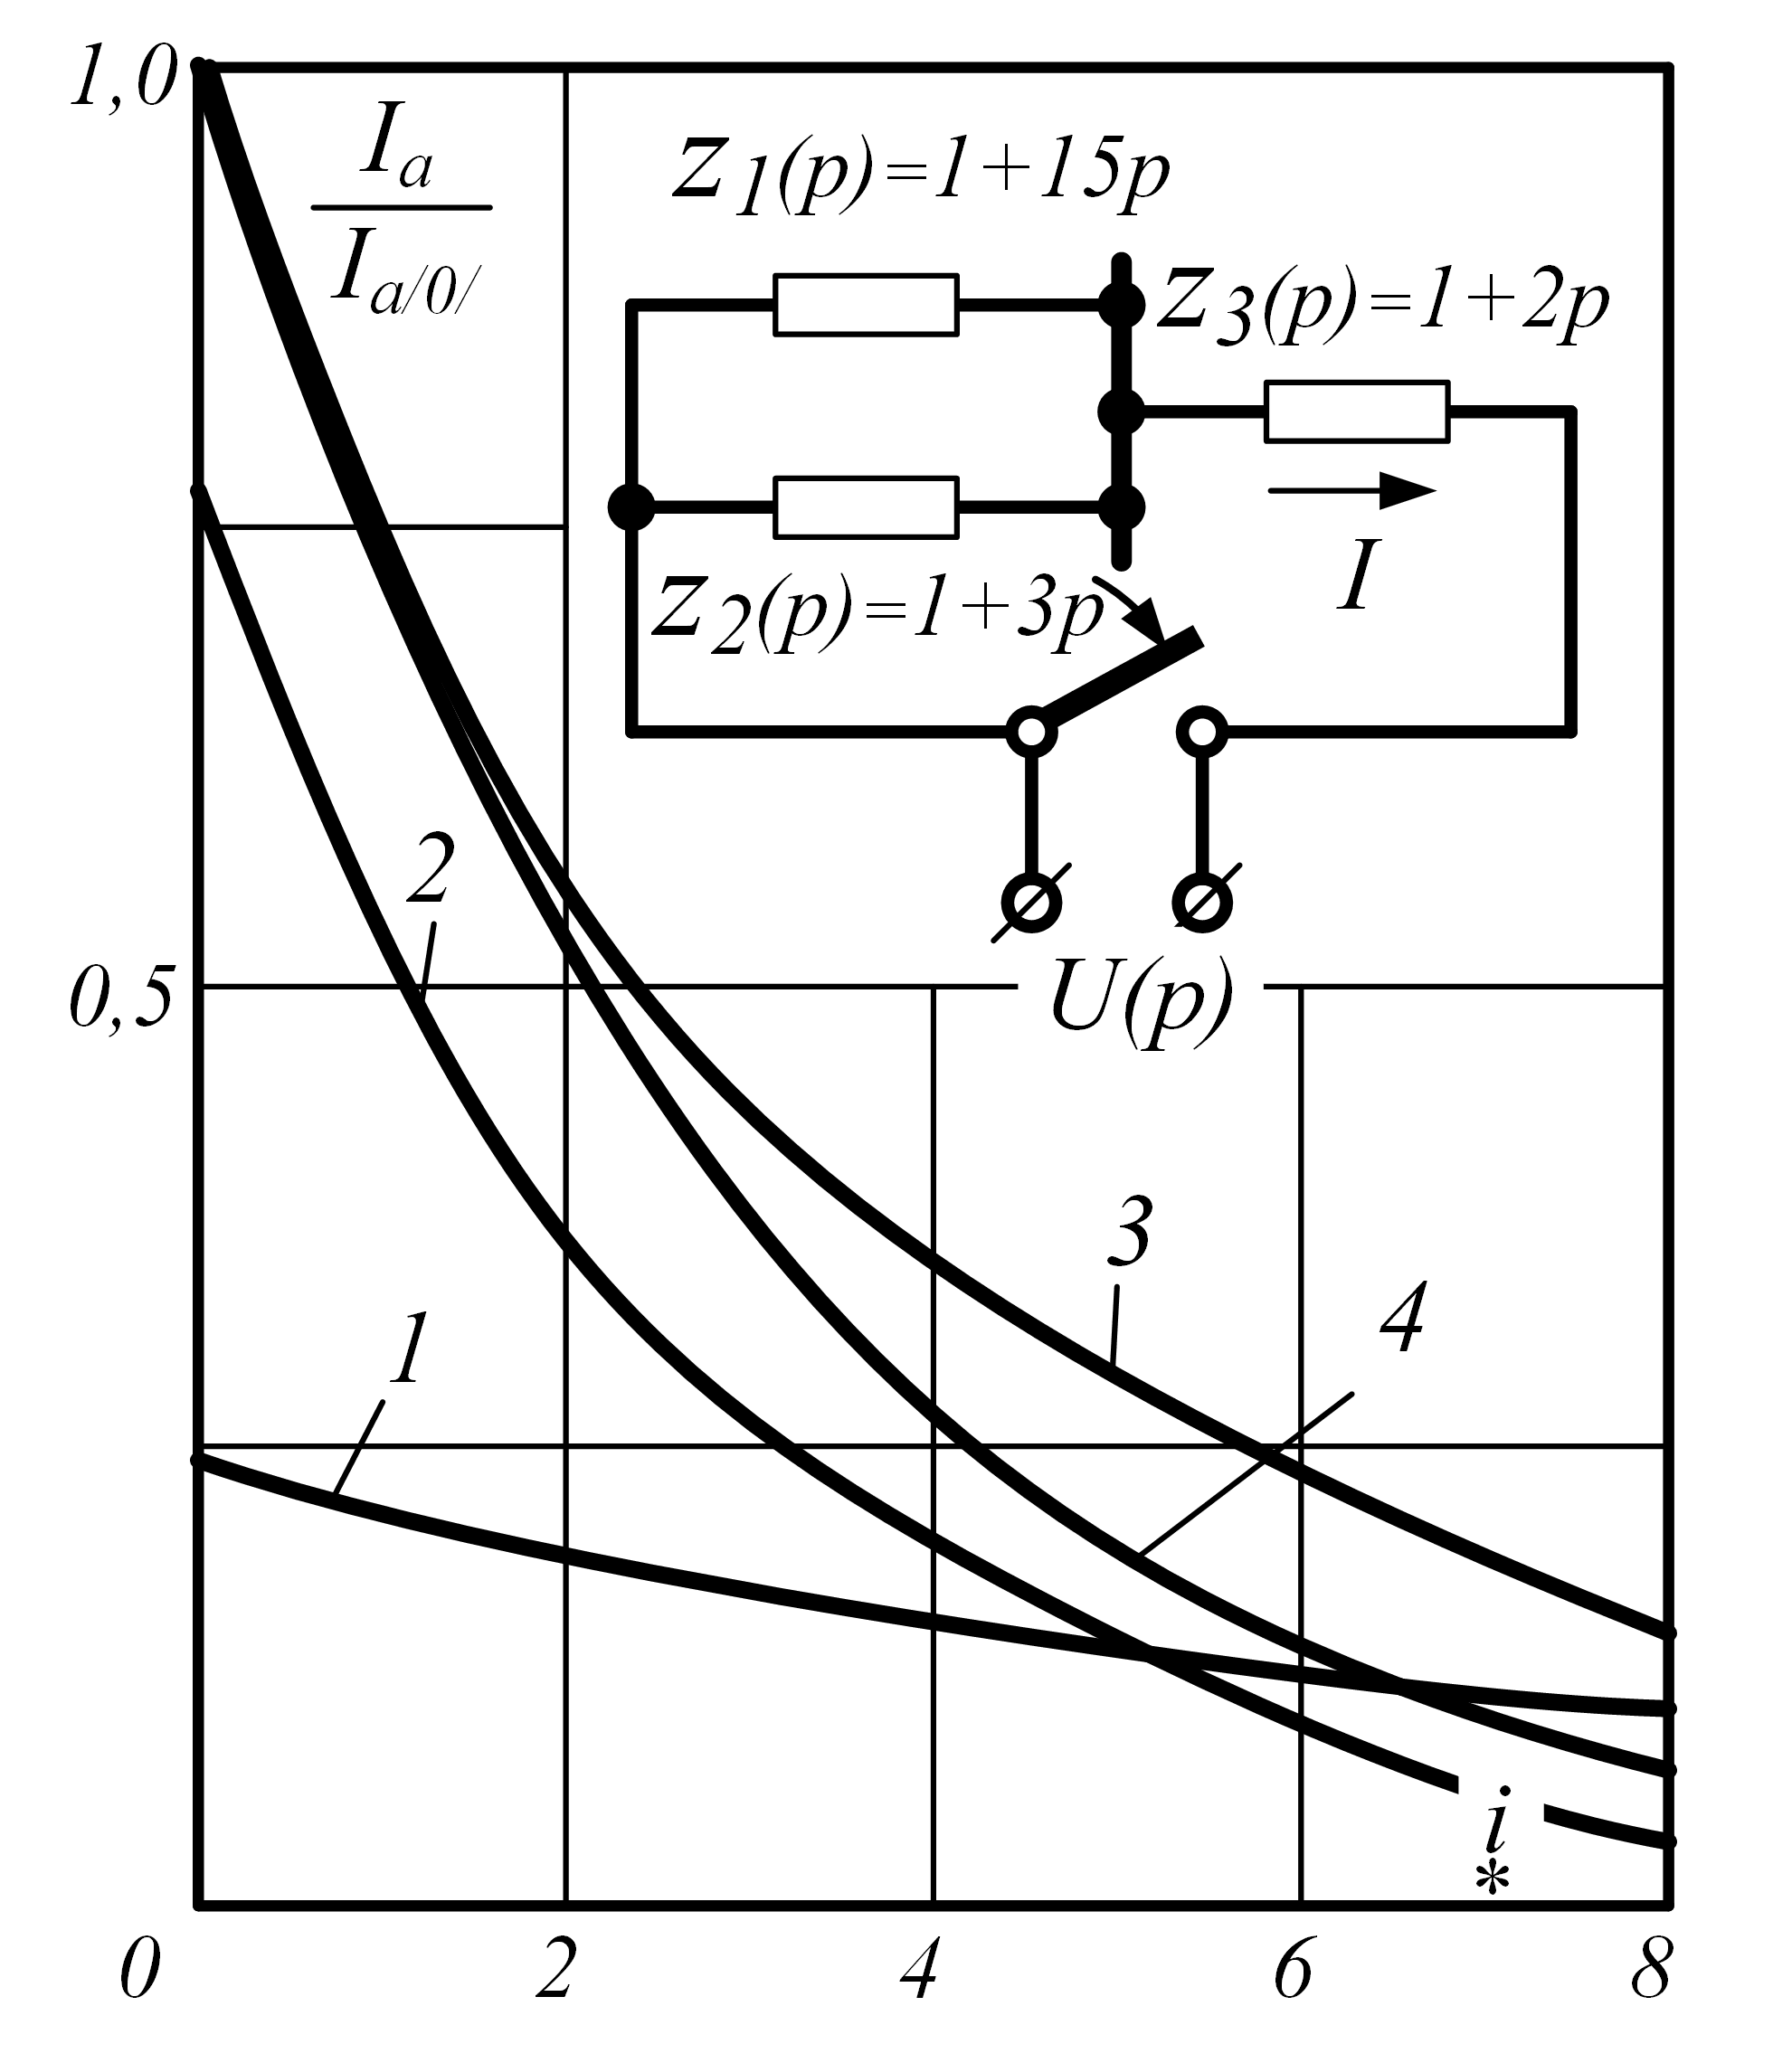
\includegraphics[width=0.7\linewidth]{pic/3-8}}
		\caption{К примеру \ref*{chap:3 perehodnyi_protcess_v_prosteishikh_trekhfaznykh_tcepiakh}-\arabic{example}. Исходная схема и кривые изменения во времени отношений токов. 
			1 --- $ I_{\text{a1}} / I_{\text{a/0/}} $;
			2 --- $ I_{\text{a2}} / I_{\text{a/0/}} $;
			3 --- $ (I_{\text{a1}} + I_{\text{a2}}) / I_{\text{a/0/}} $;
			4 --- $ I_{\text{a}} / I_{\text{a/0/}} = e^{-t/T_{\text{а.Э}}} $.}
		\label{ris:3-8 example 3-1}
	\end{figure}
	
	Используя (\ref{eq:3-14 otn}), перейдем от изображения к оригиналу:
	
	\begin{equation*}
		I_{\text{а}t} = \frac{2+18(-0,091)}{(-0,091)2 \cdot 81 (-0,091)+40}e^{-0,001t}+
		\frac{2+18(-0,405)}{(-0,405)2 \cdot 81(-0,405)+40}e^(-405t) = 
	\end{equation*}
	
	\begin{equation*}
		-0,16e^{-0,001t} -0,51e^{0,405t}.
	\end{equation*}
		
    Начальные значения частных свободных токов в долях от начального значения свободного тока в данной цени составляют:		
    
    %TODO: В книжке здесь ошибка
    \begin{equation*}
	    I_{\text{а1|0|}} = \frac{0,16}{0,16+0,51} = 0,24
	    \hspace{1pc} \text{и} \hspace{1pc}
	    I_{\text{а2|0|}} = \frac{0,51}{0,16+0,51} = 0,76.
    \end{equation*}
		
	Изменения этих токов и их суммы во времени показаны на 	рис.~\ref{ris:3-8 example 3-1}, здесь время выражено в относительных единицах.
	
	Для определения эквивалентной постоянной времени находим $ x_{\sum} $, полагая в схеме рис..~\ref{ris:3-8 example 3-1} $ r = 0 $:
	
	\begin{equation*}
		x_{\sum} = (15//3) + 2 = 4,5;
	\end{equation*}	
		
	аналогично при $ x=0 $
	
	\begin{equation*}
		r_{\sum} = \frac{1}{2} + 1 = 1,5.
	\end{equation*}	
	
	Следовательно по (\ref{eq:3-17 T_a}) находим:
	
	\begin{equation*}
		T_{\text{a.Э}} = \frac{4,5}{1,5} = 3
		\hspace{1pc} и \hspace{1pc}
		T_{\text{a.Э}} = \frac{3}{314} = 0,01 \text{~сек.}
	\end{equation*}	
	
	Экспонента этой постоянной времени представленна на рис.~\ref{ris:3-8 example 3-1} кривой \textit{4}. Ее расхождение с истинной кривой $ \frac{I_{\text{а1}}+I_{\text{а2}}}{I_{\text{а|0|}}} $ при $ \underset{*}{t} = 314 \times 0,01 = 3,14 $ (т.~е. в момент наступления максимального мгновенного значения полного тока в этой цепи) составляет примерно -10~\%.	
	
	\vspace{1pc}	
	
\end{small}


\section{Графическое решение}

Когда приложенное к цепи с $ r $ и $ L $ напряжение выражено аналитической функцией времени, решение дифференциального уравнения (\ref{eq:3-1a u}) можно выполнить, применяя, в частности, известный интеграл Дюамеля. Если же это напряжение и задано какой-либо кривой, которую нельзя представить достаточно близкой аналитической функцией, то решение уравнения (\ref{eq:3-1a u}) можно провести приближенно с помощью графического построения, основанного на следующем.

Заменим в \ref{eq:3-1a u}) производную $ di/dt $ отношением конечных разностей $ \Delta i/\Delta t $; после небольших преобразований теперь имеем:

\begin{equation}
	\frac{\Delta i}{\Delta t} = \frac{i- \frac{u}{r}}{T_{\text{а}}} = - \frac{i_{\text{св}}}{T_{\text{а}}}
	\label{eq:3-18 frac}
\end{equation}	

т.~е. скорость изменения тока в пределах интервала $ \Delta t $ пропорциональна свободному току в начале рассматриваемого интервала.

Для построения искомой кривой изменения тока во времени нужно на расстоянии $ T_{\text{а}} $ от начала координат (рис.~\ref{ris:3-9 graphic solve}) сначала нанести кривую изменения принужденного тока $ i_{\text{в}} = u/r $. Затем следует разбить ось абсцисс и кривую $ i_{\text{в}} = f(t) $ на интервалы $ \Delta t $. Для повышения точности построения целесообразно для каждого интервала использовать значение тока не в начале, а в середине интервала (точки \textit{1'}, \textit{2'}, \textit{3'},  и т.~д.). Таким образом, искомое значение тока в конце первого интервала (точка \textit{1'}) определяется пересечением соответствующей ординаты с прямой \textit{01'}, а в конце второго интервала --- пересечением соответствующей ординаты с прямой \textit{12'} и т.~д.

\begin{figure}[h]
	\center{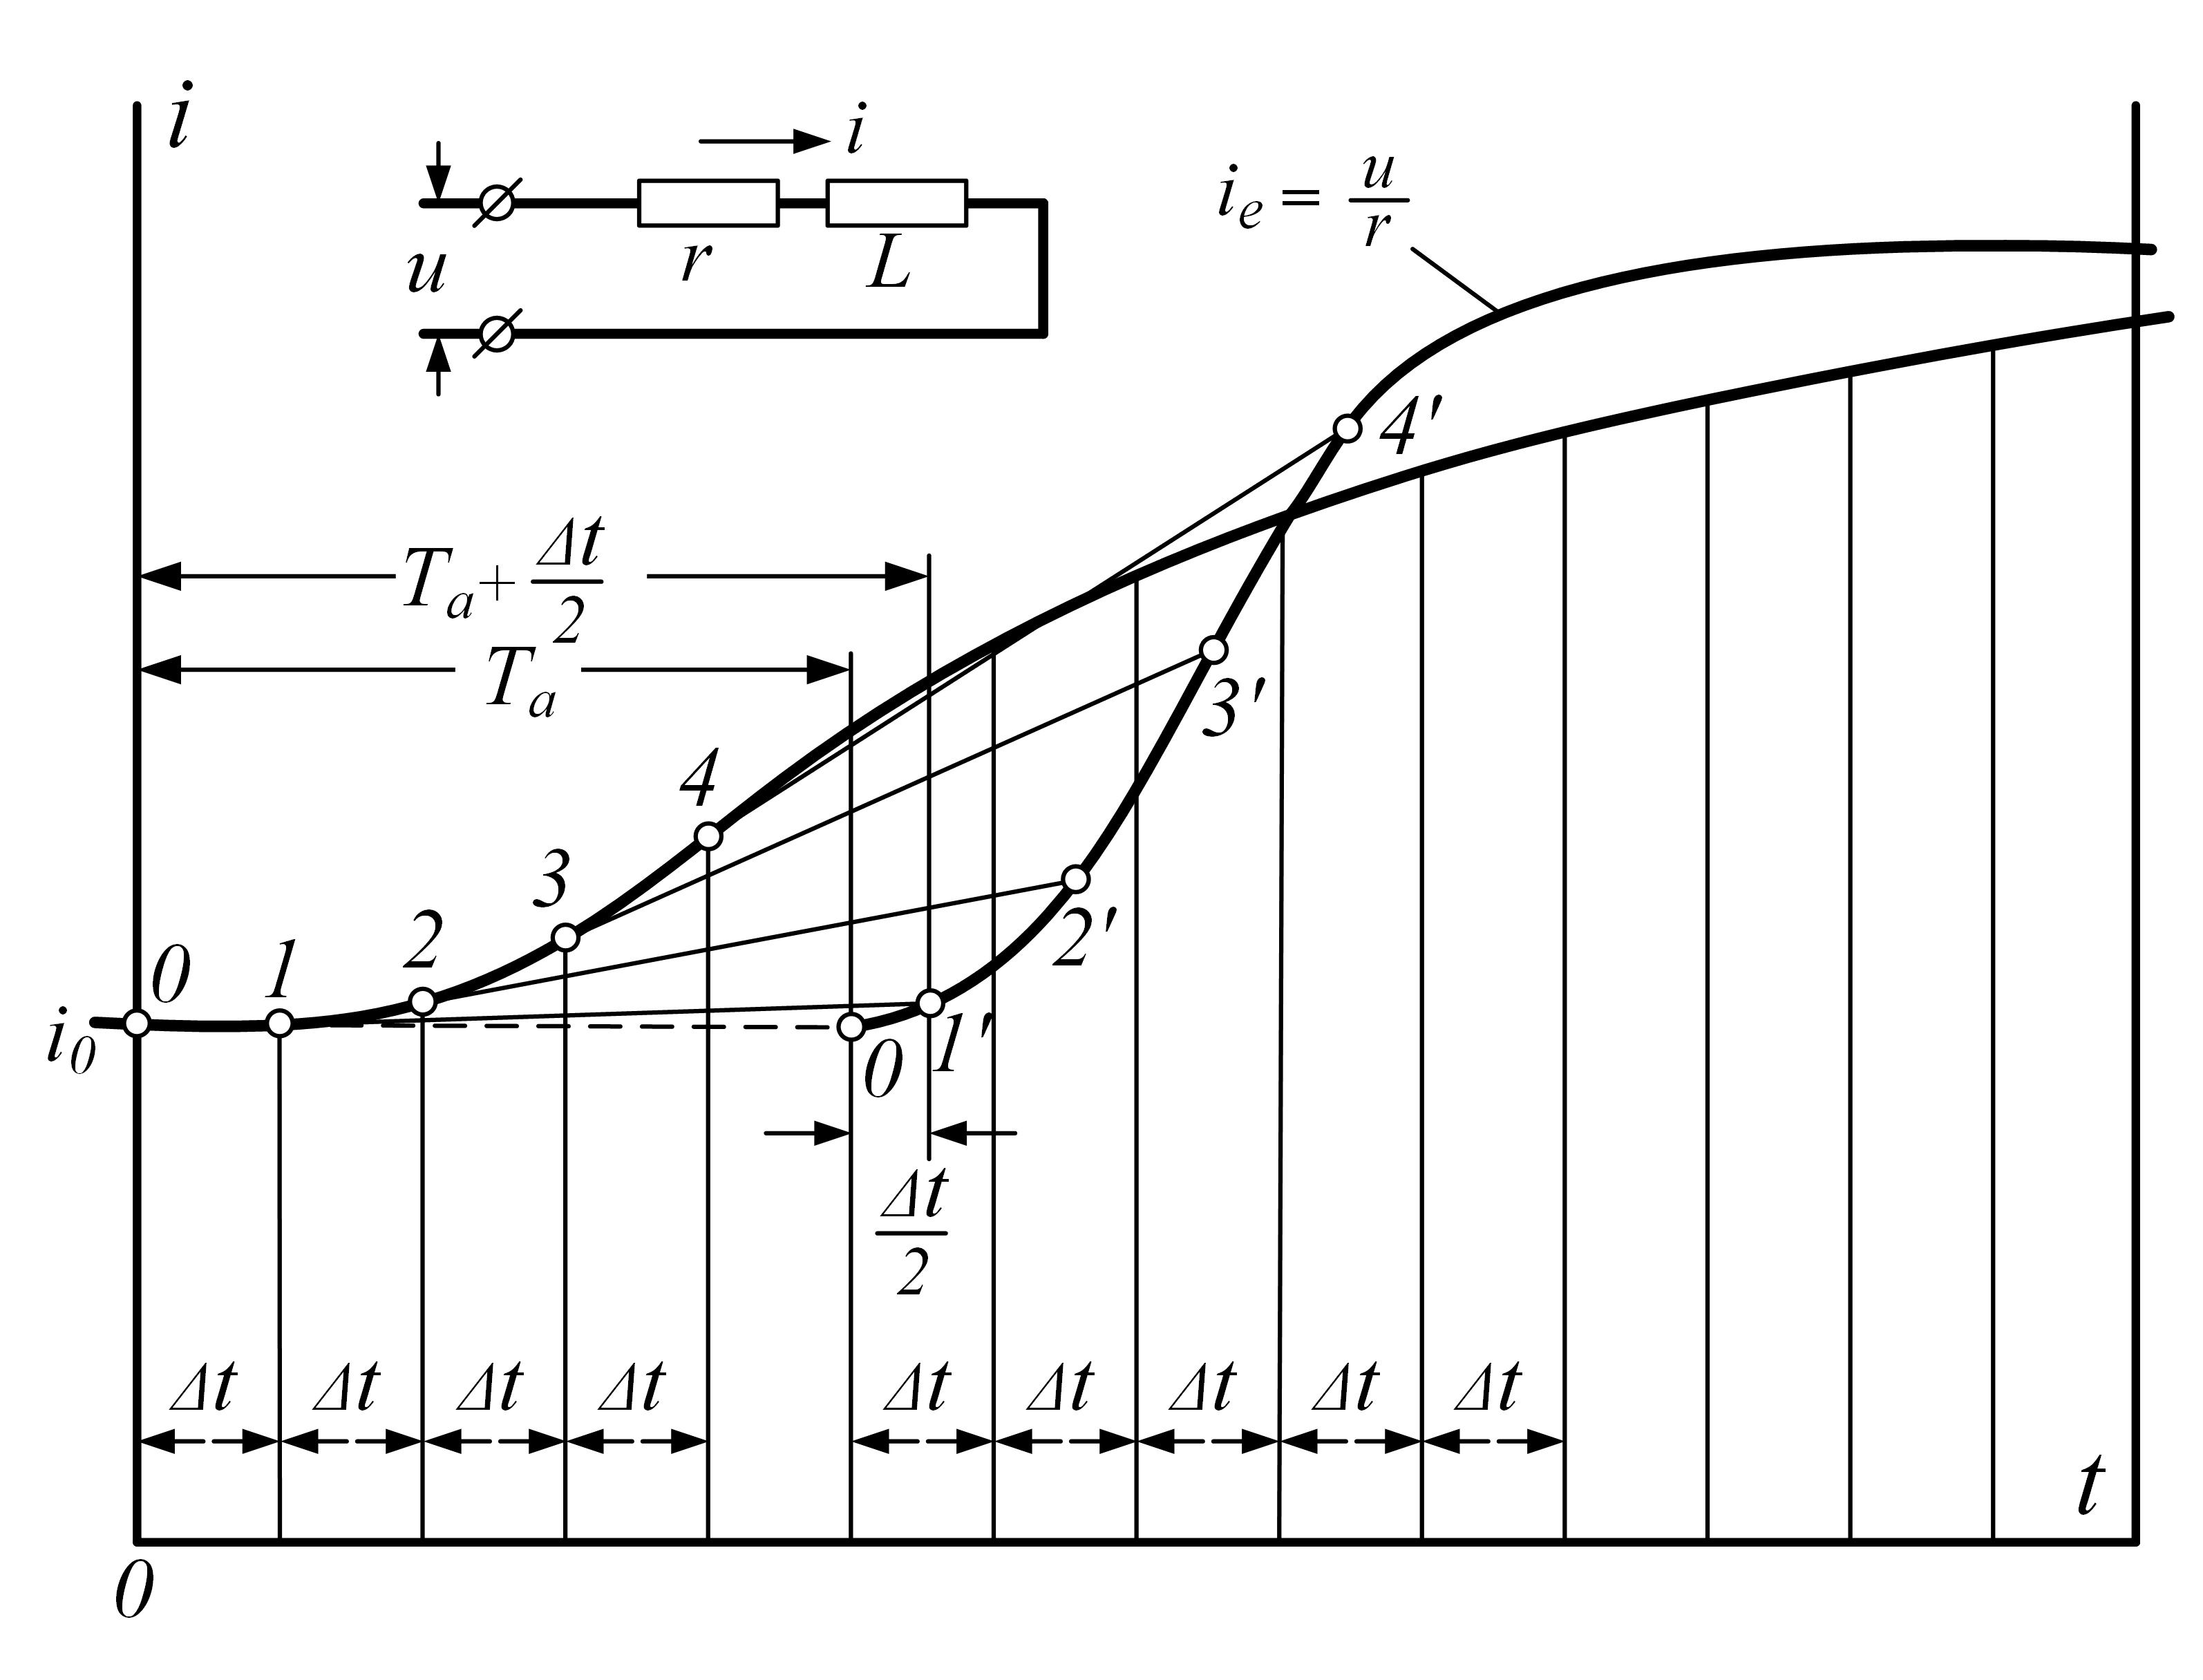
\includegraphics[width=0.7\linewidth]{pic/3-9}}
	\caption{Графический способ нахождения кривой изменения тока в цепи $ r $, $ L $, при произвольном изменении напряжения источника.}
	\label{ris:3-9 graphic solve}
\end{figure}

В зависимости от характера кривой изменения принужденной составляющей и требуемой точности решения продолжительность интервала обычно принимают в пределах $ \Delta t = 0,05 \div 0,2 $~сек.

Этот способ графического решения дифференциального уравнения вида (\ref{eq:3-1a u}) иногда используют даже в тех случаях, когда происходящее возмущение в контуре можно представить в математической форме.